\documentclass[10pt]{book}
\usepackage[utf8]{inputenc}
\usepackage[T1]{fontenc}
\usepackage{graphicx}
\usepackage{lipsum} % For dummy text
\usepackage{xcolor} % For colors
\usepackage{fancyhdr} % For header and footer customization
\usepackage{hyperref} % For hyperlinks in TOC and references
\usepackage{makeidx} % For index
\usepackage{tocloft} % For customizing TOC
\usepackage{amsmath}
\usepackage{listings}
\usepackage{xcolor}
\usepackage{hyperref}
\usepackage{appendix} % For appendix
\usepackage{biblatex} % For bibliography
\usepackage{float} % Include this in the preamble
\addbibresource{references.bib} % Bibliography file (replace references.bib with your .bib file)


%9910218400
%9899130865

% Set up header and footer
\pagestyle{fancy}
\fancyhf{}
\fancyhead[LE,RO]{\thepage}
\fancyhead[RE]{\leftmark}
\fancyhead[LO]{\rightmark}

% Customize chapter appearance
\usepackage{titlesec}
\definecolor{chaptercolor}{RGB}{51, 102, 153}
\titleformat{\chapter}[block]
  {\normalfont\Huge\bfseries\color{chaptercolor}}{\thechapter}{1em}{}

% Define color for links
\hypersetup{
    colorlinks=true,
    linkcolor=blue,
    filecolor=magenta,      
    urlcolor=cyan,
}

% For colorful Table of Contents
\renewcommand{\cftchapfont}{\color{chaptercolor}\bfseries}
\renewcommand{\cftchappagefont}{\color{chaptercolor}\bfseries}

% Index setup
\makeindex

% Begin document
\begin{document}


% Define custom color for code background and style
\definecolor{codebg}{RGB}{245,245,245}
\definecolor{codeblue}{RGB}{42, 0, 255}

\lstset{ 
    language=R, 
    backgroundcolor=\color{codebg},
    basicstyle=\ttfamily\small,
    commentstyle=\color{green!50!black},
    keywordstyle=\color{blue},
    stringstyle=\color{codeblue},
    showstringspaces=false,
    frame=single,
    rulecolor=\color{black},
    breaklines=true
}

% Front Page
\begin{titlepage}
    \centering
    \vspace*{1in}
    {\Huge\bfseries\color{chaptercolor} Applied Statistics}\\
    \vspace{0.5in}
    {\Large\textit{R Sinuvasan}}\\
    \vfill
    
\includegraphics[width=0.5\textwidth]{VIT-AP LOGO} % Replace with actual image
    \vfill
    {\Large\textbf{Department of Mathematics}}\\
    \vspace{0.2in}
    {\Large 2024}
\end{titlepage}

% Title Page (Optional)
\newpage
\thispagestyle{empty}
\begin{center}
    \vspace*{1in}
    {\Huge\bfseries\color{chaptercolor} Applied Statistics}\\
    \vspace{0.5in}
    {\Large\textit{R Sinuvasan}}\\
    \vfill
    {\Large\textbf{Department of Mathematics}}\\
    \vspace{0.2in}
    {\Large 2024}
\end{center}
\newpage

% Preface
\chapter*{Preface}
\addcontentsline{toc}{chapter}{Preface}

In today’s data-driven world, the ability to analyze and interpret data is more critical than ever. Statistics provides the foundation for understanding data, while programming tools like R offer the computational power to perform complex analyses efficiently. This manual combines essential statistical concepts with hands-on R programming, offering students a comprehensive guide to both understanding and applying statistical techniques.

This manual is designed to introduce students to fundamental statistical methods and their implementation in R, enabling them to solve real-world problems using a practical, computational approach.

The first section focuses on descriptive statistics, covering measures of central tendency such as mean, median, and mode. These tools help summarize and interpret data, providing initial insights into datasets. R functions will be introduced to calculate these measures, allowing students to immediately see how statistical concepts translate into code.

We then explore probability theory, including key concepts like random events, conditional probability, and Bayes’ theorem. With R, students will simulate probabilistic scenarios and learn how to model uncertainty using code. Bayes’ theorem, in particular, will be implemented to demonstrate how new information updates probabilities in real time.

Next, the manual covers random variables and probability distributions, both discrete and continuous. In this section, students will learn how to work with common distributions (e.g., binomial, normal, Poisson) and use R to visualize and analyze these distributions. Simulations in R will help students gain a deeper understanding of how random variables behave and how distributions are used in practice.

Understanding relationships between variables is critical in data analysis, so we explore correlation and regression analysis. Using R, students will compute correlation coefficients and build regression models to investigate the strength and direction of relationships between variables. R’s graphical capabilities will also be employed to create scatter plots, residual plots, and other visualizations, making the results more interpretable.

In the final part of the manual, we focus on decision-making through hypothesis testing. Various tests, including the z-test, t-test, F-test, and chi-square test, will be covered. Each test will be demonstrated using R, guiding students through hypothesis formulation, execution of the tests, and interpretation of results. This hands-on approach ensures that students learn not only the theory but also the practical skills necessary for conducting statistical tests using real data.

Throughout this manual, R programming is integrated seamlessly with the statistical topics covered. By the end of the course, students will have a solid understanding of both statistical theory and how to use R to implement these techniques effectively. The focus on R not only equips students with a valuable skill for the job market but also enables them to work on data-driven projects with confidence.

Each chapter contains code snippets, exercises, and case studies to reinforce learning, ensuring that students can apply their knowledge to solve real-world problems. We hope this manual serves as a valuable resource, enabling students to harness the power of statistics and R programming in their academic and professional endeavors.

This version of the preface highlights how R programming is used throughout the manual to teach statistical concepts. It emphasizes the practical, hands-on approach that students will gain by combining theory with code, preparing them for real-world data analysis tasks.
\vspace{0.5in}
R Sinuvasan \\
October 2024

\newpage

% Table of Contents
\tableofcontents
\newpage

% Chapters
\chapter{Introduction}

In an age dominated by data, the ability to analyze and interpret information has become a critical skill across various fields, including business, healthcare, social sciences, and engineering. Statistics provides the essential framework for transforming raw data into meaningful insights, enabling informed decision-making. As we navigate through complex datasets, the integration of statistical theory with programming skills has proven invaluable. Among the tools available, \textbf{R} stands out as a powerful programming language specifically designed for statistical computing and data analysis.

R is an open-source programming language that has gained immense popularity among statisticians and data scientists for its robust capabilities and extensive ecosystem. It is renowned for its ability to handle complex statistical analyses, create compelling visualizations, and manage data effectively. With a vast array of packages available—such as \texttt{dplyr} for data manipulation, \texttt{ggplot2} for data visualization, and \texttt{tidyverse} for streamlined data science workflows—R empowers users to perform sophisticated statistical analyses with relative ease. Its flexibility and adaptability make it an essential tool for anyone working with data.

This manual is structured to provide a comprehensive overview of fundamental statistical concepts while employing R programming throughout. We will explore a variety of topics that are crucial for statistical analysis, including:

\begin{itemize}
    \item \textbf{Descriptive Statistics}: We begin by examining measures of central tendency—mean, median, and mode. These statistics summarize data sets, allowing us to draw initial insights about distributions. Through R, students will learn how to calculate and visualize these measures, gaining a deeper understanding of their significance.
    
    \item \textbf{Probability Theory}: Understanding probability is essential for making predictions based on data. This section introduces key concepts, including basic probability rules, conditional probability, and Bayes’ theorem. By using R to simulate probabilistic scenarios, students will learn to model uncertainty and apply Bayes’ theorem to real-world situations, enhancing their analytical skills.
    
    \item \textbf{Random Variables and Distributions}: We will delve into random variables and their associated probability distributions, exploring both discrete and continuous cases. This section will cover important distributions such as the binomial, normal, and Poisson distributions. R will be utilized to visualize these distributions and understand their applications in statistical analysis.
    
    \item \textbf{Correlation and Regression}: Understanding relationships between variables is crucial in data analysis. We will explore correlation coefficients and regression analysis, teaching students how to quantify relationships between variables. Using R, students will create regression models and visualizations, allowing them to make predictions based on their findings.
    
    \item \textbf{Hypothesis Testing and Decision Making}: The final section addresses hypothesis testing—a fundamental aspect of statistical analysis. Students will learn how to formulate and test hypotheses using z-tests, t-tests, F-tests, and chi-square tests. R will serve as a powerful tool for conducting these tests and interpreting the results, providing students with the skills to make informed decisions based on data.
\end{itemize}

By integrating R programming throughout the manual, we ensure that students not only grasp statistical theories but also develop practical coding skills essential for data analysis. Each chapter includes coding examples, exercises, and case studies that encourage students to apply their knowledge in real-world contexts.

The use of R in this manual is supported by a wealth of literature that showcases its capabilities and applications in statistics. For instance, \textit{R for Data Science} by Hadley Wickham and Garrett Grolemund provides an excellent introduction to data science concepts using R, guiding readers through practical data analysis techniques \cite{wickham2017r}. Furthermore, the R community continuously contributes to a growing repository of packages and resources, ensuring that users have access to the latest developments in statistical methodologies.

By the end of this manual, students will have a solid foundation in both statistical concepts and R programming, equipping them with the skills necessary to tackle diverse data-driven problems. We hope this resource inspires a deeper appreciation for the power of statistics and the role of R in unlocking insights from data.




\chapter{Introduction to R Programming}

\section{Introduction to R}

R is a programming language and environment primarily used for statistical computing and data analysis. It was developed by statisticians Ross Ihaka and Robert Gentleman at the University of Auckland, New Zealand, and has gained popularity among data analysts and researchers in various fields, including social sciences, bioinformatics, and finance.

R provides a wide range of statistical techniques and is highly extensible, allowing users to create custom functions and packages. As an open-source language, R has a large and active community that continuously contributes to its development and improvement. This community-driven approach has resulted in a vast ecosystem of packages available through the Comprehensive R Archive Network (CRAN), which enhances R's capabilities for various data analysis tasks.

The language is particularly known for its powerful data visualization tools, which enable users to create high-quality graphs and plots. R's syntax and data structures are designed to facilitate data manipulation, making it a preferred choice for exploratory data analysis.

R is also widely used for reproducible research, enabling analysts to produce dynamic reports that combine code, output, and narrative text, thus making the research process transparent and verifiable. 

Overall, R has become an essential tool for data scientists and statisticians, offering robust solutions for data analysis and visualization.

\begin{itemize}
    \item History and development of R.: R was developed in the early 1990s by statisticians Ross Ihaka and Robert Gentleman at the University of Auckland, New Zealand. It was designed as a free, open-source programming language for statistical computing and data analysis, inspired by the S programming language created by John Chambers and his colleagues at Bell Laboratories.

The first version of R was released in 1995, and it quickly gained traction within the statistical community. Its development was fueled by the growing need for powerful statistical tools that were accessible to researchers and analysts. In 2000, the R Project was formally established, and R became widely recognized as a leading language for statistical analysis and data visualization.

Over the years, R has evolved significantly, with contributions from a vibrant global community of developers and users. The Comprehensive R Archive Network (CRAN) was established as a repository for R packages, allowing users to share their work and access a vast array of additional functionalities.

Today, R is supported by a comprehensive ecosystem, including numerous packages for various statistical techniques, data manipulation, and visualization. Its adoption continues to grow in academia, industry, and government, making it one of the most popular tools for data analysis and research. 

    \item Advantages of using R for statistics and data analysis.: R offers several advantages for statisticians and data analysts:

\begin{itemize}
    \item \textbf{Open Source:} R is free to use and distribute, which makes it accessible to a wide range of users and encourages community contributions.
    \item \textbf{Comprehensive Statistical Packages:} R has a vast collection of packages available through CRAN, providing tools for a wide array of statistical analyses, from basic to advanced.
    \item \textbf{Data Visualization:} R excels in data visualization, with packages like \texttt{ggplot2} that allow users to create high-quality, customizable graphics.
    \item \textbf{Active Community:} A large and active community contributes to R’s development, providing support, resources, and continuously updated packages.
    \item \textbf{Reproducible Research:} R supports reproducible research through R Markdown, allowing users to combine code, analysis, and documentation in a single document.
    \item \textbf{Integration with Other Tools:} R can easily integrate with other programming languages (e.g., Python, C++), databases, and tools, enhancing its capabilities for data analysis.
    \item \textbf{User-Friendly Syntax:} The syntax of R is designed for data analysis, making it intuitive for statisticians and researchers, even those with limited programming experience.
\end{itemize}

    \item Overview of R’s ecosystem, including RStudio and CRAN.: R's ecosystem is rich and diverse, facilitating a wide range of statistical computing and data analysis tasks. Key components include:

\begin{itemize}
    \item \textbf{R:} The core programming language, designed for statistical analysis and data manipulation, with a wide array of built-in functions and libraries.
    \item \textbf{CRAN (Comprehensive R Archive Network):} A repository of R packages that extends R’s capabilities. It hosts thousands of packages for various statistical methods, data visualization, and machine learning.
    \item \textbf{RStudio:} An integrated development environment (IDE) that enhances the R programming experience. It offers features like syntax highlighting, debugging tools, and project management, making it easier for users to write and organize their R code.
    \item \textbf{R Markdown:} A tool for creating dynamic reports that combine R code with narrative text, enabling the presentation of data analysis results in an easily shareable format.
    \item \textbf{Bioconductor:} A project that provides tools for the analysis of genomic data, offering specialized packages for bioinformatics.
    \item \textbf{Shiny:} A web application framework for R that allows users to create interactive web applications directly from R, making data analysis accessible to non-programmers.
\end{itemize}

This ecosystem collectively empowers users to perform complex data analyses, create reproducible research, and visualize results effectively.


\end{itemize}

\section{Installing R and RStudio}
To get started with R, you first need to install R and RStudio.
\begin{itemize}
    \item Step-by-step instructions for installing R and RStudio.
    \item Overview of R packages and how to install them using \texttt{install.packages()}.
    \item Basic configuration tips for RStudio.
\end{itemize}

\section{Installing R}
\subsection{Windows}
To install R on Windows:
\begin{itemize}
    \item Visit the \href{https://cran.r-project.org/bin/windows/base/}{CRAN Windows page}.
    \item Click on the download link for the latest version of R.
    \item Run the installer and follow the on-screen instructions, leaving most options at their default values unless you have specific needs.
\end{itemize}

\subsection{Mac OS X}
For Mac users:
\begin{itemize}
    \item Go to the \href{https://cran.r-project.org/bin/macosx/}{CRAN Mac OS page}.
    \item Download the most recent version of the \texttt{.pkg} file (e.g., \texttt{R-4.3.0.pkg}).
    \item Open the file and follow the installer instructions to complete the installation.
\end{itemize}

\subsection{Linux}
On Linux-based systems, R can be installed using the terminal:
\begin{itemize}
    \item Open a terminal window.
    \item For Debian-based distributions (e.g., Ubuntu), use the command:
    \begin{lstlisting}[language=R]
    sudo apt-get install r-base
    \end{lstlisting}
    \item For Fedora-based distributions, use:
    \begin{lstlisting}[language=R]
    sudo dnf install R
    \end{lstlisting}
    \item Ensure that any dependencies required by R are installed.
\end{itemize}

\section{Installing RStudio}
Once R is installed, you can install RStudio:
\begin{itemize}
    \item Visit the \href{https://www.rstudio.com/products/rstudio/download/#download}{RStudio download page}.
    \item Choose your operating system (Windows, Mac, or Linux) and download the corresponding installer.
    \item Run the installer and follow the on-screen instructions to set up RStudio.
\end{itemize}

\subsection{Windows and Mac}
For both Windows and Mac, the installation is straightforward: download the executable file, open it, and proceed with the default options unless specific configurations are needed.

\subsection{Linux}
On Linux, after downloading the \texttt{.deb} or \texttt{.rpm} file, use the terminal to install RStudio:
\begin{itemize}
    \item For Debian-based systems, run:
    \begin{lstlisting}[language=R]
    sudo dpkg -i rstudio-x.yy.zzz-amd64.deb
    \end{lstlisting}
    \item For Fedora-based systems, run:
    \begin{lstlisting}[language=R]
    sudo dnf install rstudio-x.yy.zzz-x86_64.rpm
    \end{lstlisting}
    \item Replace \texttt{x.yy.zzz} with the actual version number of RStudio you downloaded.
\end{itemize}

\section{Overview of R Packages}
R packages are collections of R functions, data, and compiled code that are stored in a well-defined format. They extend R's functionality by providing tools for specific tasks, such as data manipulation, visualization, or statistical analysis. Many packages are available through CRAN (Comprehensive R Archive Network), but others are hosted on platforms like GitHub.

\section{Installing R Packages}
To install an R package, use the \texttt{install.packages()} function. This function downloads and installs the specified package from CRAN or other repositories.

\subsection{Example of Installing a Package}
For example, to install the \texttt{ggplot2} package for data visualization, run the following command in your R console:
\begin{lstlisting}[language=R]
install.packages("ggplot2")
\end{lstlisting}
This command will download and install the package, including any dependencies, automatically.

\subsection{Loading an Installed Package}
Once a package is installed, load it into your R session using the \texttt{library()} function:
\begin{lstlisting}[language=R]
library(ggplot2)
\end{lstlisting}

\section{Commonly Used Packages}
Some widely-used packages in R include:
\begin{itemize}
    \item \texttt{dplyr} – for data manipulation
    \item \texttt{ggplot2} – for data visualization
    \item \texttt{tidyverse} – a collection of data science tools
    \item \texttt{shiny} – for building interactive web applications
\end{itemize}




\section{Basic Configuration Tips for RStudio}
\begin{itemize}
    \item \textbf{Appearance:} Go to \texttt{Tools > Global Options > Appearance} to change the editor theme and font size for better visibility.
    \item \textbf{Pane Layout:} Customize the layout of RStudio panes (Source, Console, Environment) under \texttt{Tools > Global Options > Pane Layout}.
\end{itemize}

\section{Code Execution}
\begin{itemize}
    \item Enable line numbers, auto-complete, and code folding under \texttt{Tools > Global Options > Code}.
    \item Set keyboard shortcuts for running code chunks (e.g., \texttt{Ctrl + Enter}).
\end{itemize}

\section{Packages}
\begin{itemize}
    \item Manage installed packages via the \texttt{Packages} tab or use \texttt{install.packages()} to add new packages.
\end{itemize}





\section{Basic R Syntax}
Understanding the basic syntax of R is crucial for efficient programming.
\begin{itemize}
    \item Variables, data types (numeric, character, factor, logical).
    \item Basic operators (arithmetic, relational, logical).
    \item Introduction to vectors and data frames.
\end{itemize}





\section{Variables in R}
Variables in R are used to store data that can be manipulated during the execution of a program. A variable can be assigned a value using the assignment operator \texttt{<-} or \texttt{=}. For example:
\begin{lstlisting}[language=R]
x <- 10
name <- "John"
\end{lstlisting}
In R, variables do not need explicit declaration, and their type is determined dynamically when a value is assigned.

\section{Data Types in R}
R provides several basic data types that are essential for handling different kinds of data. These include numeric, character, factor, and logical types.

\subsection{Numeric}
The numeric data type is used to store numbers, both integers and real numbers (decimals). For example:
\begin{lstlisting}[language=R]
x <- 42
y <- 3.14
\end{lstlisting}
R treats all numbers as double precision by default, but integers can also be explicitly declared using the \texttt{as.integer()} function.

\subsection{Character}
Character data represents text or strings. Characters are enclosed in double or single quotes. For example:
\begin{lstlisting}[language=R]
name <- "Alice"
greeting <- 'Hello'
\end{lstlisting}

\subsection{Factor}
Factors are used to handle categorical data in R. They store both the values and the possible categories. Factors are particularly useful for statistical modeling:
\begin{lstlisting}[language=R]
colors <- factor(c("red", "blue", "green", "red"))
\end{lstlisting}
Factors can be ordered or unordered and are often used in data frames for analysis.

\subsection{Logical}
Logical data types store boolean values: \texttt{TRUE} or \texttt{FALSE}. They are often the result of comparisons or logical operations:
\begin{lstlisting}[language=R]
is_sunny <- TRUE
result <- 5 > 3  # result will be TRUE
\end{lstlisting}


Understanding variables and data types is crucial for working effectively with R. The dynamic nature of R allows for flexible handling of different types of data, making it easier to perform statistical analysis and data manipulation.







\section{Introduction}
In R, operators allow you to perform various computations on data. These include arithmetic operations for numerical calculations, relational operators for comparisons, and logical operators for evaluating boolean expressions. Understanding these operators is fundamental for programming in R.

\section{Arithmetic Operators}
Arithmetic operators are used for basic mathematical computations. The main arithmetic operators in R are:
\begin{itemize}
    \item \texttt{+} : Addition
    \item \texttt{-} : Subtraction
    \item \texttt{*} : Multiplication
    \item \texttt{/} : Division
    \item \texttt{\^} : Exponentiation
    \item \texttt{\%/\%} : Integer division (quotient)
    \item \texttt{\%\%} : Modulo (remainder)
\end{itemize}



\subsection{Examples}
\begin{lstlisting}[language=R]
x <- 10
y <- 3

sum <- x + y        # sum = 13
diff <- x - y       # diff = 7
prod <- x * y       # prod = 30
quot <- x / y       # quot = 3.33
exp <- x ^ y        # exp = 1000
int_div <- x %/% y  # int_div = 3
mod <- x %% y       # mod = 1
\end{lstlisting}

\section{Relational Operators}
Relational operators compare values and return \texttt{TRUE} or \texttt{FALSE}. The main relational operators are:
\begin{itemize}
    \item \texttt{==} : Equal to
    \item \texttt{!=} : Not equal to
    \item \texttt{>} : Greater than
    \item \texttt{<} : Less than
    \item \texttt{>=} : Greater than or equal to
    \item \texttt{<=} : Less than or equal to
\end{itemize}

\subsection{Examples}
\begin{lstlisting}[language=R]
x <- 5
y <- 10

result1 <- x == y    # result1 = FALSE
result2 <- x != y    # result2 = TRUE
result3 <- x > y     # result3 = FALSE
result4 <- x <= y    # result4 = TRUE
\end{lstlisting}

Relational operators are often used in conditions for \texttt{if} statements, loops, and other control structures.

\section{Logical Operators}
Logical operators evaluate logical expressions and are primarily used to combine relational operations. The main logical operators are:
\begin{itemize}
    \item \texttt{\&} : Logical AND
    \item \texttt{|} : Logical OR
    \item \texttt{!} : Logical NOT
\end{itemize}

\subsection{Examples}
\begin{lstlisting}[language=R]
a <- TRUE
b <- FALSE

result1 <- a & b     # result1 = FALSE (both must be TRUE)
result2 <- a | b     # result2 = TRUE (one must be TRUE)
result3 <- !a        # result3 = FALSE (logical negation)
\end{lstlisting}

Logical operators are especially useful when you need to check multiple conditions.


Arithmetic, relational, and logical operators are crucial in R for data manipulation, decision-making, and computations. They provide a foundation for writing effective R scripts and performing complex analyses.




\section{Vectors in R}
A vector is one of the most basic data structures in R. It is a sequence of data elements of the same type, such as numeric, character, or logical. Vectors can be created using the \texttt{c()} function, which combines values into a single vector.

\subsection{Example of a Numeric Vector}
\begin{lstlisting}[language=R]
numbers <- c(1, 2, 3, 4, 5)
\end{lstlisting}
Vectors in R are 1-dimensional and are fundamental to most data manipulation operations.

\subsection{Example of a Character Vector}
\begin{lstlisting}[language=R]
names <- c("Alice", "Bob", "Charlie")
\end{lstlisting}



In this chapter, we will cover vectors. A vector is a data structure in R. A data structure can be defined as a collection of data values, the relationships among them, and the functions or operations that can be applied to the data. A vector can either be an atomic vector or a list. An atomic vector contains only one data type, whereas a list may contain multiple data types.

An atomic vector could be Character, Logical, Double, Integer, or Complex.

\subsection{Integer}
\begin{lstlisting}[language=R]
4
## [1] 4
\end{lstlisting}

\subsection{Character}
\begin{lstlisting}[language=R]
"Pune"
## [1] "Pune"
\end{lstlisting}

You can use the \texttt{typeof} function to check the type of each of these:
\begin{lstlisting}[language=R]
typeof("Pune")
## [1] "character"
typeof(4)
## [1] "double"
typeof(4.3)
## [1] "double"
typeof(2+1i) 
## [1] "complex"
\end{lstlisting}

\subsection{Creating a Vector}
Let's create a vector containing three numeric values. This will be an example of a Numeric Vector:
\begin{lstlisting}[language=R]
c(1, 4, 7)
## [1] 1 4 7
\end{lstlisting}

To check the length of the vector, we can use the length function:
\begin{lstlisting}[language=R]
length(c(1, 4, 7))
## [1] 3
\end{lstlisting}

Let's assign this to a variable for future use:
\begin{lstlisting}[language=R]
Num_variable <- c(1, 4, 7)
\end{lstlisting}

Let’s create a vector \texttt{Names} that contains the names of persons appearing in an Exam. This will be a kind of character vector. Please note that here \texttt{Names} is a vector, and \texttt{<-} is an operator that assigns the value on the right-hand side of the operator to the variable name on the left-hand side. The character \texttt{c} is used to create a vector:
\begin{lstlisting}[language=R]
Names <- c("Arvind", "Krishna", "Rahul", "Saurabh", "Venkat", "Sucharitha")
\end{lstlisting}

Let's extract the first element of the \texttt{Names} vector. To extract the first element, we need to use \texttt{[} and the value 1:
\begin{lstlisting}[language=R]
Names[1]
## [1] "Arvind"
\end{lstlisting}

Similarly, to extract the third value from the \texttt{Names} vector:
\begin{lstlisting}[language=R]
Names[3]
## [1] "Rahul"
\end{lstlisting}

Let’s create another vector and see if we can combine two vectors:
\begin{lstlisting}[language=R]
Missed_names <- c("Ajay", "Amit")
\end{lstlisting}

Here we will be updating the \texttt{Names} vector by including \texttt{Missed\_names} in the \texttt{Names} vector:
\begin{lstlisting}[language=R]
Names <- c(Names, Missed_names)
Names
## [1] "Arvind"     "Krishna"    "Rahul"      "Saurabh"    "Venkat"    
## [6] "Sucharitha" "Ajay"       "Amit"
\end{lstlisting}

\subsection{Class of Vector}
We can also check the types of vectors using different functions such as:
\begin{lstlisting}[language=R]
class(Names)
## [1] "character"
class(Num_variable)
## [1] "numeric"
typeof(Num_variable)
## [1] "double"
\end{lstlisting}

What is the difference between \texttt{typeof}, \texttt{mode}, and \texttt{class}? I will leave it to the reader to explore it on their own. Remember the reader can use the \texttt{help} function to check the definitions in detail. For example, just type \texttt{?class} in the console to see the details of the class function.

\subsection{Adding Vectors of Different Types}
Let’s add a character and numeric vector and check the result:
\begin{lstlisting}[language=R]
mix_vector <- c(1, 2, "Amish")
class(mix_vector)
## [1] "character"
\end{lstlisting}

The \texttt{mix\_vector} we created had multiple data types (Numeric and Character); however, R converts the multiple data types to a single data type through a process called coercion. Logical values are converted to numbers: TRUE is converted to 1 and FALSE to 0.

Values are converted to the simplest type required to represent all information.

The ordering is roughly logical < integer < numeric < complex < character < list.

Objects of type \texttt{raw} are not converted to other types.

Objects can also be explicitly coerced using the \texttt{as.} function. For example, to coerce the \texttt{mix\_vector} to numeric use:
\begin{lstlisting}[language=R]
mix_vector <- as.numeric(mix_vector)
## Warning: NAs introduced by coercion
mix_vector
## [1]  1  2 NA
class(mix_vector)
## [1] "numeric"
\end{lstlisting}

We can also change the elements of the vector. Let’s change the first element of the \texttt{Names} vector using the following expression:
\begin{lstlisting}[language=R]
Names[1] <- "Arun"
Names
## [1] "Arun"       "Krishna"    "Rahul"      "Saurabh"    "Venkat"    
## [6] "Sucharitha" "Ajay"       "Amit"
\end{lstlisting}

\subsection{Accessing Elements of Vectors}
Let’s try to access elements of the vector using negative indexing:
\begin{lstlisting}[language=R]
Names[-1] # All elements except the first element will be printed
## [1] "Krishna"    "Rahul"      "Saurabh"    "Venkat"     "Sucharitha"
## [6] "Ajay"       "Amit"
Names[c(-1, -2)] # All elements except the first and second elements will be printed
## [1] "Rahul"      "Saurabh"    "Venkat"     "Sucharitha" "Ajay"      
## [6] "Amit"
\end{lstlisting}

Alternatively, we can also use the following code to remove the first two elements of the \texttt{Names} vector:
\begin{lstlisting}[language=R]
Names[-c(1, 2)] # All elements except the first and second elements will be printed
## [1] "Rahul"      "Saurabh"    "Venkat"     "Sucharitha" "Ajay"      
## [6] "Amit"
\end{lstlisting}

\subsection{Creating Vector Using In-Built Functions}
\begin{lstlisting}[language=R]
seq(1, 10, by = 1) # Create a sequential vector from 1 to 10 which increases by 1 in length.
##  [1]  1  2  3  4  5  6  7  8  9 10
seq(1, 10, by = 0.5)
##  [1]  1.0  1.5  2.0  2.5  3.0  3.5  4.0  4.5  5.0  5.5  6.0  6.5  7.0  7.5
## [15]  8.0  8.5  9.0  9.5 10.0
\end{lstlisting}

\subsection{Let’s Try to Repeat Vectors}
\begin{lstlisting}[language=R]
rep(c(1, 2), times = c(5, 5))
##  [1] 1 1 1 1 1 2 2 2 2 2
\end{lstlisting}

\texttt{typeof(Vector)}: This method tells you the data type of the vector.

\texttt{Sort(Vector)}: This method helps us to sort the items in ascending order.

\texttt{length(Vector)}: This method counts the number of elements in a vector.

\texttt{head(Vector, limit)}: This method returns the top six elements (if you omit the limit). If you specify the limit as 4, then it returns the first 4 elements.

\texttt{tail(Vector, limit)}: It returns the last six elements (if you omit the limit). If you specify the limit as 2, then it returns the last two elements.

\subsection{Arithmetic Operators in Vectors in R}

We have performed arithmetic operations in previous chapters. Let’s see how we can perform arithmetic operations in vectors.

\begin{lstlisting}[language=R]
V1 <- c(1, 2, 3, 4) # created a vector V1 
V2 <- c(5, 6, 7, 8) # created a vector V2
\end{lstlisting}

Let's perform addition:
\begin{lstlisting}[language=R]
V12 <- V1 + V2
V12 # Print result of V12, which is sum of V1 and V2 vector.
## [1]  6  8 10 12
\end{lstlisting}

As you may have guessed, the addition operation above was performed elementwise. That means that the first element of \texttt{V1} was added to the first element of \texttt{V2}.

Let’s perform multiplication:
\begin{lstlisting}[language=R]
V12_mult <- V1 * V2
V12_mult
## [1]  5 12 21 32
\end{lstlisting}

Let’s perform division:
\begin{lstlisting}[language=R]
V12_division <- V2 / V1
V12_division
## [1] 5.000000 3.000000 2.333333 2.000000
typeof(V12_division)
## [1] "double"
\end{lstlisting}

Let’s convert the double to numeric:
\begin{lstlisting}[language=R]
V12_division <- as.integer(V12_division)
V12_division
## [1] 5 3 2 2
typeof(V12_division)
## [1] "integer"
\end{lstlisting}







%\section{Data Frames in R}
%A data frame is a table or a 2-dimensional array-like structure in which each column contains values of one variable, and each row represents an observation. Each column can have different data types, making data frames essential for handling datasets in R.
%
%\subsection{Creating a Data Frame}
%\begin{lstlisting}[language=R]
%df <- data.frame(Name = c("Alice", "Bob"), Age = c(25, 30))
%\end{lstlisting}
%Data frames are widely used for data analysis, especially when handling structured datasets such as those found in spreadsheets.
%
%
%Vectors and data frames are foundational data structures in R. Vectors store sequences of the same data type, while data frames are ideal for storing datasets with different types across columns.
%
%
%
%
%
%
%\section{Data Frames}
%Understanding data frames as a primary data structure in R.
%\begin{itemize}
%    \item Creating data frames and manipulating them using \texttt{data.frame()} and related functions.
%    \item Accessing and subsetting data frames.
%\end{itemize}
%
%\section{Matrices}
%Introduction to matrices as a data structure in R.
%\begin{itemize}
%    \item Creating matrices using \texttt{matrix()}, and performing operations.
%    \item Differences between matrices and data frames.
%\end{itemize}



\section{Introduction to Data Frames in R}

Data frames in R language are a type of data structure used to store data in a tabular form, which is two-dimensional. The data frames are a special category of list data structures in which the components are of equal length. R language supports the built-in function \texttt{data.frame()} to create data frames and assign data elements. R also supports using the data frame name to modify and retrieve data elements from data frames. Data frames in R are structured with column names as component names, and rows structured by component values. Data frames in R are a widely used data structure when developing machine learning models in data science projects.

\subsection{Characteristics of Data Frames}
\begin{itemize}
    \item The column name is required.
    \item Row names should be unique.
    \item The number of items in each column should be the same.
\end{itemize}

\section{Steps For Creating Data Frames in R}

Let’s start with creating a data frame, which is explained below:

\subsection{Step 1: Create a Data Frame of a Class in a School}
\textbf{Code:}
\begin{lstlisting}[language=R]
tenthclass = data.frame(roll_number = c(1:5),
Name = c("John","Sam","Casey","Ronald","Mathew"),
Marks = c(77,87,45,68,95), stringsAsFactors = FALSE)
print(tenthclass)
\end{lstlisting}

When we run this code, we will get a data frame like this:

\textbf{Output:}

\begin{figure}[h]
    \begin{flushleft}
        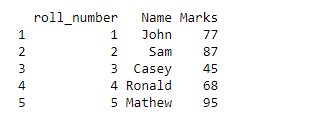
\includegraphics[width=0.7\textwidth]{Data-Frames-in-R-1-1.png} % Image file
        \caption{Data frame output example}
        \label{fig:dataframe}
    \end{flushleft}
\end{figure}
Here, in our example, the data frame is very small, but in real life, while dealing with problems, we have lots of data. To understand the structure of the data, we use the \texttt{Str()} function.

\subsection{Step 2: Add the following line to our code}

\textbf{Code:}
\begin{lstlisting}[language=R]
Str(tenthclass)
\end{lstlisting}

When we run the whole code, we will get the following output:

\textbf{Output:}
\begin{figure}[h]
    \begin{flushleft}
        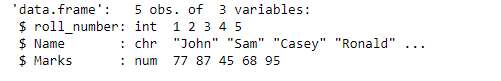
\includegraphics[width=0.7\textwidth]{Data-Frames-in-R-1-2.png} % Image file
        \caption{Data frame output example}
        \label{fig:dataframe}
    \end{flushleft}
\end{figure}

The above output means we have 5 observations of 3 variables. It also explains the data type of each variable. For example, the roll number is an integer, the name is a character, and Marks are numeric.

Once we understand the structure of the data, we can pass the following code to understand the data more statistically.

\subsection{Step 3: Use the \texttt{summary()} Function}

\textbf{Code:}
\begin{lstlisting}[language=R]
summary(tenthclass)
\end{lstlisting}

\textbf{Output:}
\begin{figure}[h]
    \begin{flushleft}
        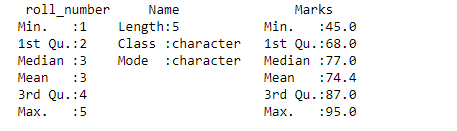
\includegraphics[width=0.7\textwidth]{Data-Frames-in-R-1-3.png} % Image file
        \caption{Data frame output example}
        \label{fig:dataframe}
    \end{flushleft}
\end{figure}

The \texttt{summary()} function provides a better understanding of our data. It tells us the mean, median, quartiles, maximum, and minimum values, helping us make better decisions.



\section*{Structure}
When we want to know the structure of a particular data frame, we can use the following function:

\begin{lstlisting}[language=R]
Star()

str(Data_frame)
\end{lstlisting}

\noindent Output:

\begin{lstlisting}[language=R]
Number: num  2 3 4
alpha: Factor w/ 3 levels “x”,”y”,”z”: 1 2 3
Booleans: logi  TRUE TRUE FALSE
\end{lstlisting}


\section*{How to Extract Data from Data Frames in R?}
Here we will continue the above case. Let’s suppose we want to know the name of the student in class tenth, just the name. So how will we extract it?

Our data frame looks like this:

\begin{lstlisting}[language=R]
roll_number   Name   Marks
1             John   77
2             Sam    87
3             Casey  45
4             Ronald 68
5             Mathew 95
\end{lstlisting}

To just get the name as an output, we will pass on the following code.

\subsection*{Code:}
\begin{lstlisting}[language=R]
onlyname = tenthclass$Name
print(onlyname)
\end{lstlisting}

\textbf{Output:}
\begin{figure}[H]
    \begin{flushleft}
        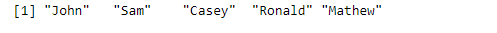
\includegraphics[width=0.7\textwidth]{Data-Frames-in-R-1-4.png}
        \caption{Data frame output example}
        \label{fig:dataframe}
    \end{flushleft}
\end{figure}

Here, if we break the code, we just put the dollar sign in between the name of our data frame and the name of the variable that we want as an output.

Now consider a situation: the teacher wants to know everything about roll number 2, like what his name is and how much he scored.

We need everything about roll number 2, so we will pass on the below-mentioned code.

\subsection*{Code:}
\begin{lstlisting}[language=R]
result_rollnumber2 = tenthclass[c(2), c(1:3)]
print(result_rollnumber2)
\end{lstlisting}

\noindent Output:
\begin{figure}[H]
    \begin{flushleft}
        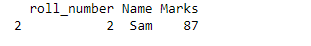
\includegraphics[width=0.7\textwidth]{Data-Frames-in-R-1-5.png}
        \caption{Data frame output example}
        \label{fig:dataframe}
    \end{flushleft}
\end{figure}

\subsection*{Expand in Data Frames}
The data frame can be increased and decreased in size by adding or deleting columns and rows.

\subsubsection*{1. Add Row}
We have two data frames. One data frame belongs to class tenth section A and the other data frame belongs to class tenth section B. Now these different sections are merging into a single class.

\paragraph{Example \#1: Class 10 A}
\subsection*{Code:}
\begin{lstlisting}[language=R]
tenthclass_sectionA = data.frame(roll_number = c(1:5),
Name = c("John","Sam","Casey","Ronald","Mathew"),
Marks = c(77,87,45,68,95), stringsAsFactors = FALSE)
print(tenthclass_sectionA)
\end{lstlisting}

\noindent Output:
\begin{figure}[H]
    \begin{flushleft}
        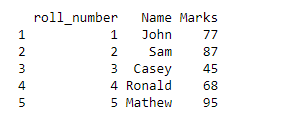
\includegraphics[width=0.7\textwidth]{Data-Frames-in-R-1-6.png}
        \caption{Data frame output example}
        \label{fig:dataframe}
    \end{flushleft}
\end{figure}


\paragraph{Example \#2: Class 10 B}
\subsection*{Code:}
\begin{lstlisting}[language=R]
tenthclass_sectionB = data.frame(roll_number = c(6:10),
Name = c("Ria","Justin","Bon","Tim","joe"),
Marks = c(68,98,54,68,42), stringsAsFactors = FALSE)
print(tenthclass_sectionB)
\end{lstlisting}

\noindent Output:
\begin{figure}[H]
    \begin{flushleft}
        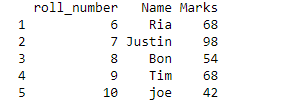
\includegraphics[width=0.7\textwidth]{Data-Frames-in-R-1-7.png}
        \caption{Data frame output example}
        \label{fig:dataframe}
    \end{flushleft}
\end{figure}
\paragraph{Example \#3: rbind() function}
Now we have to merge both classes into a single class. We will use the \texttt{rbind()} function here. The only limitation in adding a new row is that we need to bring in the new rows in the same structure as the existing data frame.

\subsection*{Code:}
\begin{lstlisting}[language=R]
new_tenthclass = rbind(tenthclass_sectionA, tenthclass_sectionB)
print(new_tenthclass)
\end{lstlisting}

\noindent Output:
\begin{figure}[H]
    \begin{flushleft}
        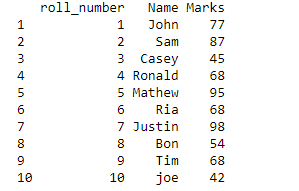
\includegraphics[width=0.7\textwidth]{Data-Frames-in-R-1-8.png}
        \caption{Data frame output example}
        \label{fig:dataframe}
    \end{flushleft}
\end{figure}

\subsubsection*{2. Add Column}
Now consider a case where we have to add blood group details for every student in class 10. We will add a new column for it and name it as “Blood\_group”.

Our data frame looks like this:

\subsection*{Code:}
\begin{lstlisting}[language=R]
tenthclass = data.frame(roll_number = c(1:5),
Name = c("John","Sam","Casey","Ronald","Mathew"),
Marks = c(77,87,45,68,95), stringsAsFactors = FALSE)
print(tenthclass)
\end{lstlisting}

\noindent Output:
\begin{figure}[H]
    \begin{flushleft}
        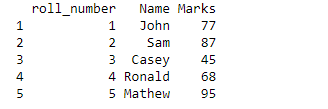
\includegraphics[width=0.7\textwidth]{Data-Frames-in-R-1-9.png}
        \caption{Data frame output example}
        \label{fig:dataframe}
    \end{flushleft}
\end{figure}

\subsection*{Code:}
\begin{lstlisting}[language=R]
tenthclass$Blood_group = c("O","AB","B+","A+","AB")
print(tenthclass)
\end{lstlisting}

\noindent Output:
\begin{figure}[H]
    \begin{flushleft}
        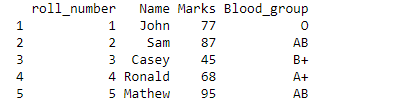
\includegraphics[width=0.7\textwidth]{Data-Frames-in-R-1-10.png}
        \caption{Data frame output example}
        \label{fig:dataframe}
    \end{flushleft}
\end{figure}

\subsubsection*{3. Delete Column}
In this data frame, if we need to delete the blood group variable (the rightmost column), we will pass the following code.

\subsection*{Code:}
\begin{lstlisting}[language=R]
tenthclass$Blood_group = NULL
print(tenthclass)
\end{lstlisting}

\noindent Output:
\begin{figure}[H]
    \begin{flushleft}
        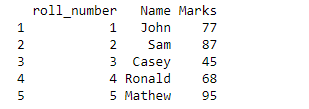
\includegraphics[width=0.7\textwidth]{Data-Frames-in-R-1-12.png}
        \caption{Data frame output example}
        \label{fig:dataframe}
    \end{flushleft}
\end{figure}

By passing the \texttt{NULL} command, we can directly remove the variable from our data frame.

\subsubsection*{4. Delete Row}
Now consider a situation where we don’t need the marks of John, so we have to remove the topmost row.

\subsection*{Code:}
\begin{lstlisting}[language=R]
tenthclass = tenthclass[-1, ]
print(tenthclass)
\end{lstlisting}

\noindent Output:
\begin{figure}[H]
    \begin{flushleft}
        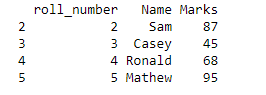
\includegraphics[width=0.7\textwidth]{Data-Frames-in-R-1-14.png}
        \caption{Data frame output example}
        \label{fig:dataframe}
    \end{flushleft}
\end{figure}
\subsubsection*{5. Update Data in Data Frame}
Let’s suppose Sam scored 98 marks, but in our data frame, his marks are shown as 87. We can pass the following code to rectify this.

\subsection*{Code:}
\begin{lstlisting}[language=R]
tenthclass$Marks[2] = 98
print(tenthclass)
\end{lstlisting}

\noindent Output:
\begin{figure}[H]
    \begin{flushleft}
        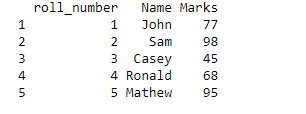
\includegraphics[width=0.7\textwidth]{Data-Frames-in-R-1-16.png}
        \caption{Data frame output example}
        \label{fig:dataframe}
    \end{flushleft}
\end{figure}



\section{Inspecting Data Frames}
Below are different ways to inspect a data frame and obtain information about it, similar to the \texttt{str()} function.

\subsection*{1. Names: Provides the Names of the Variables in the Data Frame}
\textbf{Syntax}:
\begin{lstlisting}[language=R]
names(data_frame_name)
\end{lstlisting}

\textbf{Example}:
\begin{lstlisting}[language=R]
Number <- c(2,3,4)
alpha <- c("x","y","z")
Booleans <- c(TRUE,TRUE,FALSE)
Data_frame <- data.frame(Number, alpha, Booleans)
names(Data_frame)
\end{lstlisting}

\textbf{Output}:
\begin{lstlisting}[language=R]
[1] "Number" "alpha" "Booleans"
\end{lstlisting}

\subsection*{2. Summary: Provides Statistics of the Data Frame}
\textbf{Syntax}:
\begin{lstlisting}[language=R]
summary(data_frame_name)
\end{lstlisting}

\textbf{Example}:
\begin{lstlisting}[language=R]
Number <- c(2,3,4)
alpha <- c("x","y","z")
Booleans <- c(TRUE,TRUE,FALSE)
Data_frame <- data.frame(Number, alpha, Booleans)
summary(Data_frame)
\end{lstlisting}

\textbf{Output}:
\begin{lstlisting}[language=R]
     Number     alpha   Booleans
 Min.   :2.0   x:1     Mode :logical
 1st Qu.:2.5   y:1     FALSE:1
 Median :3.0   z:1     TRUE :2
 Mean   :3.0   NA’s:0
 3rd Qu.:3.5
 Max.   :4.0
\end{lstlisting}

\subsection*{3. Head: Provides the Data for the First Few Rows}
\textbf{Syntax}:
\begin{lstlisting}[language=R]
head(data_frame_name)
\end{lstlisting}

\textbf{Example}:
\begin{lstlisting}[language=R]
Number <- c(2,3,4,5,6,7,8,9,10,11)
alpha <- c("x","y","z","a","b","c","d","f","g","j")
Booleans <- c(TRUE,TRUE,FALSE,TRUE,FALSE,FALSE,FALSE,FALSE,FALSE,FALSE)
Data_frame <- data.frame(Number, alpha, Booleans)
head(Data_frame)
\end{lstlisting}

\textbf{Output}:
\begin{lstlisting}[language=R]
Number alpha Booleans
1      2      x     TRUE
2      3      y     TRUE
3      4      z     FALSE
4      5      a     TRUE
5      6      b     FALSE
6      7      c     FALSE
\end{lstlisting}

\subsection*{4. Tail: Prints the Last Few Rows in the Data Frame}
\textbf{Syntax}:
\begin{lstlisting}[language=R]
tail(data_frame_name)
\end{lstlisting}

\textbf{Example}:
\begin{lstlisting}[language=R]
Number <- c(2,3,4,5,6,7,8,9,10,11)
alpha <- c("x","y","z","a","b","c","d","f","g","j")
Booleans <- c(TRUE,TRUE,FALSE,TRUE,FALSE,FALSE,FALSE,FALSE,FALSE,FALSE)
Data_frame <- data.frame(Number, alpha, Booleans)
tail(Data_frame)
\end{lstlisting}

\textbf{Output}:
\begin{lstlisting}[language=R]
Number alpha Booleans
5      6      b    FALSE
6      7      c    FALSE
7      8      d    FALSE
8      9      f    FALSE
9     10      g    FALSE
10    11      j    FALSE
\end{lstlisting}

\section{Extracting Specific Data from the Data Frame}
\subsection*{1. Using the Column Name}
We can extract a particular set of data from the data frame. For instance, to extract only the \texttt{Number} column:

\begin{lstlisting}[language=R]
Data_frame <- data.frame(Number)
\end{lstlisting}

\textbf{Output}:
\begin{lstlisting}[language=R]
Number
1      2
2      3
3      4
\end{lstlisting}

\subsection*{2. Using the Rows}
To print only the first two rows of the \texttt{Number} column:

\begin{lstlisting}[language=R]
output <- Data_frame[1:2,]
print(output)
\end{lstlisting}

\textbf{Output}:
\begin{lstlisting}[language=R]
Number alpha Booleans
1      2      x     TRUE
2      3      y     TRUE
\end{lstlisting}

\subsection*{3. Printing Specific Rows and Columns}
For example, to print rows 1 and 2 of columns 1 and 2:

\begin{lstlisting}[language=R]
output <- Data_frame[c(1,2),c(1,2)]
print(output)
\end{lstlisting}

\textbf{Output}:
\begin{lstlisting}[language=R]
Number alpha
1      2     x
2      3     y
\end{lstlisting}

\subsection*{4. Adding Another Column to the Data Frame}
\begin{lstlisting}[language=R]
Data_frame$class <- c("A","B","C")
\end{lstlisting}

\textbf{Output}:
\begin{lstlisting}[language=R]
Number alpha Booleans class
1      2     x     TRUE     A
2      3     y     TRUE     B
3      4     z    FALSE     C
\end{lstlisting}

\subsection*{5. Adding a Row to the Data Frame}
We use \texttt{rbind()} to add a new row:

\begin{lstlisting}[language=R]
out <- rbind(Data_frame, c(5, "x", FALSE, "D"))
print(out)
\end{lstlisting}

\textbf{Output}:
\begin{lstlisting}[language=R]
Number alpha Booleans class
1      2     x     TRUE     A
2      3     y     TRUE     B
3      4     z    FALSE     C
4      5     x    FALSE     D
\end{lstlisting}

\subsection*{6. Combining Both Data Frames}
\begin{lstlisting}[language=R]
out <- rbind(Data_frame1, Data_frame2)
print(out)
\end{lstlisting}

\textbf{Output}:
\begin{lstlisting}[language=R]
Number alpha Booleans
1      2      x    TRUE
2      3      y    TRUE
3      4      z   FALSE
4      4      x    TRUE
5      5      y    TRUE
6      6      z   FALSE
\end{lstlisting}

\section{Conclusion}
Data frames are commonly used data structures that list variables with unique row IDs. This article covers methods for adding and deleting rows and columns, updating data, and accessing data in a data frame.








\section{Matrices in R}

Matrices are two-dimensional data structures in R and are arranged in a rectangular layout. Matrices can contain only one data type. We can create matrices of any of the six data types we discussed before. A matrix can also be thought of as a vector in two dimensions.

We can use the \texttt{matrix} function to create a matrix in R programming. I will suggest using \texttt{? matrix} for detailed documentation of the matrix function. Let’s create a matrix with 3 rows and 2 columns:

\begin{lstlisting}[language=R]
matrix(1:6, nrow = 3, ncol = 2)
##      [,1] [,2]
## [1,]    1    4
## [2,]    2    5
## [3,]    3    6
\end{lstlisting}

What if we don’t specify the number of rows and columns?

\begin{lstlisting}[language=R]
matrix(1:6, 3, 2)
##      [,1] [,2]
## [1,]    1    4
## [2,]    2    5
## [3,]    3    6
\end{lstlisting}

As you have guessed from the above output, R will automatically pick the number of rows and columns based on the order of input. Let’s specify one of the dimensions (either column or row) and see the output:

\begin{lstlisting}[language=R]
matrix(1:6, ncol = 3)
##      [,1] [,2] [,3]
## [1,]    1    3    5
## [2,]    2    4    6
\end{lstlisting}

So far we have not assigned any column names and row names to the matrix. Let’s create a matrix \( M \) and assign column names and row names:

\begin{lstlisting}[language=R]
M <- matrix(1:20, ncol = 4)
colnames(M) <- c("A", "B", "C", "D")
rownames(M) <- c("E", "F", "G", "H", "I")
\end{lstlisting}

Let’s check the matrix \( M \):

\begin{lstlisting}[language=R]
M
##   A  B  C  D
## E 1  6 11 16
## F 2  7 12 17
## G 3  8 13 18
## H 4  9 14 19
## I 5 10 15 20
\end{lstlisting}

As you can see from the output, we have successfully assigned names to the columns. We can also call specific columns now. For example, \texttt{Matrix[rowname, colname]} will call the required row and column by name:

\begin{lstlisting}[language=R]
M["F", "D"]
## [1] 17
\end{lstlisting}

We can leave the row name field blank in \texttt{Matrix[rowname, colname]} to call the complete column:

\begin{lstlisting}[language=R]
M[, "D"]
##  E  F  G  H  I 
## 16 17 18 19 20
\end{lstlisting}

As you can see in the above example, we have kept the row blank. This will cause the above expression to pick all the values from the corresponding columns. We can also access specific elements of vectors by specifying the row number and column number. Let’s say we want to pick a specific column and vector from matrix, say the 2nd row and 3rd column:

\begin{lstlisting}[language=R]
M[2, 3]
## [1] 12
\end{lstlisting}

\subsection{Extracting Row/Column from Matrices}

We can also extract more than one row or column at a time. For example, below we extracted the first and third column and the second row:

\begin{lstlisting}[language=R]
M[2, c(1, 3)]
##  A  C 
##  2 12
\end{lstlisting}

So what else can we do with matrices?

\subsection{Operations in Matrices}

Let’s perform some operations with matrices. Let’s create two matrices \( M_1 \) and \( M_2 \) and perform some operations:

\begin{lstlisting}[language=R]
M1 <- matrix(1:15, nrow = 5)
M1
##      [,1] [,2] [,3]
## [1,]    1    6   11
## [2,]    2    7   12
## [3,]    3    8   13
## [4,]    4    9   14
## [5,]    5   10   15

M2 <- matrix(1:15, nrow = 5)
M2
##      [,1] [,2] [,3]
## [1,]    1    6   11
## [2,]    2    7   12
## [3,]    3    8   13
## [4,]    4    9   14
## [5,]    5   10   15
\end{lstlisting}

\subsubsection{Arithmetic Operations in Matrices}

What if we add two matrices? Matrix operations can be performed similarly to how arithmetic operations are performed on numbers. However, we should be careful with the dimensions of the matrices that we are working on.

Let’s create three matrices \( M_1, M_2, M_3 \):

\begin{lstlisting}[language=R]
M1 <- matrix(1:15, nrow = 5)
M1
##      [,1] [,2] [,3]
## [1,]    1    6   11
## [2,]    2    7   12
## [3,]    3    8   13
## [4,]    4    9   14
## [5,]    5   10   15

M2 <- matrix(2:16, nrow = 5)
M2
##      [,1] [,2] [,3]
## [1,]    2    7   12
## [2,]    3    8   13
## [3,]    4    9   14
## [4,]    5   10   15
## [5,]    6   11   16

M3 <- matrix(2:10, nrow = 5)
## Warning in matrix(2:10, nrow = 5): data length [9] is not a sub-multiple or
## multiple of the number of rows [5]
M3
##      [,1] [,2]
## [1,]    2    7
## [2,]    3    8
## [3,]    4    9
## [4,]    5   10
## [5,]    6    2
\end{lstlisting}

\textbf{Arithmetic Operations in Matrices}

Addition operation on matrices of the same dimension:

\begin{lstlisting}[language=R]
M1 + M2
##      [,1] [,2] [,3]
## [1,]    3   13   23
## [2,]    5   15   25
## [3,]    7   17   27
## [4,]    9   19   29
## [5,]   11   21   31
\end{lstlisting}

What if we want to add matrices of different dimensions? We can check the dimensions of matrices using the \texttt{dim} function:

\begin{lstlisting}[language=R]
dim(M1)
## [1] 5 3
dim(M3)
## [1] 5 2
\end{lstlisting}

Multiplying matrices of the same dimension: The following operation using \texttt{"*"} is element-wise:

\begin{lstlisting}[language=R]
M1 * M2
##      [,1] [,2] [,3]
## [1,]    2   42  132
## [2,]    6   56  156
## [3,]   12   72  182
## [4,]   20   90  210
## [5,]   30  110  240
\end{lstlisting}
What if we want Matrix Multiplication? As an exercise, try \texttt{M1\%*\%M2} in the R console for matrix multiplication and check the result. Once you run the operation, you must have got an error message ``Error in M1 \%*\% M2: non-conformable arguments". Why is it so? As a basic rule for matrix multiplication, the number of rows of Matrix1 should be equal to the number of columns in Matrix2 when multiplying Matrix1 with Matrix2. You can check the following link \textit{mathisfun}.

\begin{lstlisting}[language=R]
M4 <- matrix(1:9, nrow=3)
M5 <- matrix(10:18, nrow=3)
M4
\end{lstlisting}
\begin{lstlisting}[language=R]
##      [,1] [,2] [,3]
## [1,]    1    4    7
## [2,]    2    5    8
## [3,]    3    6    9
\end{lstlisting}
\begin{lstlisting}[language=R]
M5
\end{lstlisting}
\begin{lstlisting}[language=R]
##      [,1] [,2] [,3]
## [1,]   10   13   16
## [2,]   11   14   17
## [3,]   12   15   18
\end{lstlisting}
Let's see the result of Matrix Multiplication:

\begin{lstlisting}[language=R]
M4 <- matrix(1:9, nrow=3)
M5 <- matrix(10:18, nrow=3)
M4 \%*\% M5
\end{lstlisting}
\begin{lstlisting}[language=R]
##      [,1] [,2] [,3]
## [1,]  138  174  210
## [2,]  171  216  261
## [3,]  204  258  312
\end{lstlisting}
You can see the elementwise operation result in R:

\begin{lstlisting}[language=R]
M4 * M5
\end{lstlisting}
\begin{lstlisting}[language=R]
##      [,1] [,2] [,3]
## [1,]   10   52  112
## [2,]   22   70  136
## [3,]   36   90  162
\end{lstlisting}
\begin{lstlisting}[language=R]
M1 / M2
\end{lstlisting}
\begin{lstlisting}[language=R]
##           [,1]      [,2]      [,3]
## [1,] 0.5000000 0.8571429 0.9166667
## [2,] 0.6666667 0.8750000 0.9230769
## [3,] 0.7500000 0.8888889 0.9285714
## [4,] 0.8000000 0.9000000 0.9333333
## [5,] 0.8333333 0.9090909 0.9375000
\end{lstlisting}
What if one of the matrices' row or column is shorter than the other? Will recycling occur?

As an exercise, create a 3X3 matrix and add it to M1.

\subsection{Transposing a Matrix}
You may also want to transpose your data in R. This is used to interchange rows and columns, i.e., rows become columns and columns become rows in the new transposed matrix. For example:

\begin{lstlisting}[language=R]
M3 <- t(M1)
M3
\end{lstlisting}
\begin{lstlisting}[language=R]
##      [,1] [,2] [,3] [,4] [,5]
## [1,]    1    2    3    4    5
## [2,]    6    7    8    9   10
## [3,]   11   12   13   14   15
\end{lstlisting}
As you can see from the output, the rows have become columns and the columns have become rows. This can also be used to reshape a DataFrame. We will cover DataFrame in the next chapter.

\subsection{Common Matrix Operations in R}
Sum of rows in Matrix:
\begin{lstlisting}[language=R]
rowSums(M1)
\end{lstlisting}
\begin{lstlisting}[language=R]
## [1] 18 21 24 27 30
\end{lstlisting}

Sum of columns in Matrix:
\begin{lstlisting}[language=R]
colSums(M1)
\end{lstlisting}
\begin{lstlisting}[language=R]
## [1] 15 40 65
\end{lstlisting}

Mean of rows in Matrix:
\begin{lstlisting}[language=R]
rowMeans(M1)
\end{lstlisting}
\begin{lstlisting}[language=R]
## [1]  6  7  8  9 10
\end{lstlisting}

\subsection{Naming Matrix Rows and Columns}
\begin{lstlisting}[language=R]
rownames(M4) <- c("A","B","C")
colnames(M4) <- c("D","E","F")
M4
\end{lstlisting}
\begin{lstlisting}[language=R]
##   D E F
## A 1 4 7
## B 2 5 8
## C 3 6 9
\end{lstlisting}

We can also extract specific elements of a Matrix by specifying rows and columns:

\begin{lstlisting}[language=R]
M4[3,] % # Extracting third row from Matrix M4
\end{lstlisting}
\begin{lstlisting}[language=R]
## D E F 
## 3 6 9
\end{lstlisting}
\begin{lstlisting}[language=R]
M4[,3] % # Extracting third column from Matrix M4
\end{lstlisting}
\begin{lstlisting}[language=R]
## A B C 
## 7 8 9
\end{lstlisting}
\begin{lstlisting}[language=R]
M4[2,3] % # Extracting second row and third column element from Matrix M4
\end{lstlisting}
\begin{lstlisting}[language=R]
## [1] 8
\end{lstlisting}











\section{Creating a Function}
In R, functions are created using the \texttt{function} keyword. They take arguments as input, perform specified operations, and return a result. The structure is:

\begin{lstlisting}
function_name <- function(arg1, arg2 = default_value, ...) {
    # Function body with operations
    return(result)
}
\end{lstlisting}

\section{Function Arguments}
Arguments are inputs for functions, and R supports several types:
\begin{itemize}
    \item \textbf{Positional Arguments}: Matched in the order defined.
    \item \textbf{Named Arguments}: Specified by name; order doesn't matter.
    \item \textbf{Default Arguments}: Take predefined values unless overwritten.
    \item \textbf{Flexible Arguments (\texttt{...})}: Allow a variable number of inputs.
\end{itemize}

\subsection{Example with Default and Named Arguments}
\begin{lstlisting}
calculate_area <- function(length, width = 5) {
    area <- length * width
    return(area)
}
calculate_area(3)          # Uses default width = 5
calculate_area(3, width = 4) # Overwrites default width with 4
\end{lstlisting}

\section{Return Values}
Functions can return values explicitly with \texttt{return()}, or implicitly by using the last evaluated expression. They can return multiple values via lists.

\begin{lstlisting}
multi_return <- function(x) {
    sum_x <- sum(x)
    mean_x <- mean(x)
    return(list(sum = sum_x, mean = mean_x))
}
result <- multi_return(c(1, 2, 3, 4))
\end{lstlisting}

\section{Default Arguments}
Default arguments allow certain parameters to be optional.

\begin{lstlisting}
greet <- function(name = "User") {
    paste("Hello,", name)
}
greet()          # Output: "Hello, User"
greet("Alice")   # Output: "Hello, Alice"
\end{lstlisting}

\section{Lazy Evaluation}
R uses lazy evaluation, meaning arguments are only evaluated when needed.

\begin{lstlisting}
lazy_eval <- function(x, y) {
    if (x > 0) {
        return(x * y)
    } else {
        return("x is not greater than zero")
    }
}
\end{lstlisting}

\section{Anonymous Functions}
Anonymous functions, or functions without names, are used for short operations, such as with \texttt{apply} functions.

\begin{lstlisting}
numbers <- list(1, 2, 3, 4)
squares <- lapply(numbers, function(x) x^2)
\end{lstlisting}

\section{Scoping Rules}
R uses lexical scoping, which searches for variables starting from the local environment.

\begin{lstlisting}
x <- 10
scope_example <- function(y) {
    x <- 5
    return(x + y)
}
scope_example(3)  # Returns 8; local x = 5 is used
\end{lstlisting}

\section{Complete Example of a Function}
The following example shows various components, such as arguments, control flow, and list returns.

\begin{lstlisting}
generate_report <- function(data, show_summary = TRUE, ...) {
    if (!is.data.frame(data)) stop("Data must be a data frame")
    
    if (show_summary) {
        summary_data <- summary(data, ...)
        print("Summary Statistics:")
        print(summary_data)
    }
    
    num_data <- data[sapply(data, is.numeric)]
    mean_values <- sapply(num_data, mean, ...)
    
    return(list(summary = summary_data, means = mean_values))
}
generate_report(mtcars)
\end{lstlisting}

\section{Conclusion}
Functions in R provide a powerful and flexible way to perform calculations, customize analyses, and structure code. They are essential for creating reusable, organized, and efficient code.









\section{Data Import and Export in R}
Data import is a crucial aspect of data analysis, as it enables R to read and manipulate various data formats. Here’s a breakdown of common data file types and methods for importing them:

\subsection{1. CSV Files}
CSV files are among the most widely used formats for data storage. They contain plain text data organized in a tabular format, where each line corresponds to a row and each value is separated by a comma.

\textbf{Functionality:} The \texttt{read.csv()} function is tailored for reading CSV files. It automatically assumes that the first line contains header names, making it convenient for typical datasets.

\textbf{Example:}
\begin{lstlisting}[language=R]
data <- read.csv("data.csv", header = TRUE, sep = ",")
\end{lstlisting}

\textbf{Parameters:}
\begin{itemize}
    \item \texttt{header}: Logical value indicating whether the first row contains column names.
    \item \texttt{na.strings}: A character vector of strings to interpret as NA values.
    \item \texttt{stringsAsFactors}: If TRUE, converts character vectors to factors.
\end{itemize}

\subsection{2. Excel Files}
Excel is another common format for data storage, particularly in business and research settings. R provides the \texttt{readxl} package to read Excel files (.xls and .xlsx).

\textbf{Functionality:} The \texttt{read\_excel()} function allows users to specify which sheet to read.

\textbf{Example:}
\begin{lstlisting}[language=R]
library(readxl)
data <- read_excel("data.xlsx", sheet = "Sheet1")
\end{lstlisting}

\textbf{Parameters:}
\begin{itemize}
    \item \texttt{col\_names}: Set to TRUE or FALSE to indicate whether to treat the first row as column names.
    \item \texttt{range}: Allows users to specify a particular range of cells to import.
\end{itemize}

\subsection{3. Text Files}
For text files that may not conform to the CSV format, R provides \texttt{read.table()} and \texttt{read.delim()} for more control.

\textbf{Functionality:} \texttt{read.table()} is flexible, allowing you to specify any delimiter.

\textbf{Example:}
\begin{lstlisting}[language=R]
data <- read.table("data.txt", header = TRUE, sep = "\t")
\end{lstlisting}

\textbf{Parameters:}
\begin{itemize}
    \item \texttt{quote}: Specify character(s) to treat as quotes.
    \item \texttt{fill}: If TRUE, will fill rows with fewer columns with NA.
\end{itemize}

\subsection{4. R Data Files}
R provides the ability to save objects in its own binary format, useful for saving complex objects.

\textbf{Functionality:} The \texttt{load()} function loads R objects stored in .RData files.

\textbf{Example:}
\begin{lstlisting}[language=R]
load("data.RData")
\end{lstlisting}

\subsection{5. Databases}
R can connect to various database systems (like MySQL, PostgreSQL, and SQLite) through the \texttt{DBI} package.

\textbf{Functionality:} You can execute SQL queries to read data directly from databases.

\textbf{Example:}
\begin{lstlisting}[language=R]
library(DBI)
con <- dbConnect(RSQLite::SQLite(), dbname = "database.db")
data <- dbReadTable(con, "table_name")
\end{lstlisting}

\subsection{6. SPSS, SAS, and Stata Files}
For users working with data from statistical software, the \texttt{haven} package enables importing data from formats like SPSS (.sav), SAS (.sas7bdat), and Stata (.dta).

\textbf{Functionality:} Functions like \texttt{read\_sav()}, \texttt{read\_dta()}, and \texttt{read\_sas()} make it easy to read these files.

\textbf{Example:}
\begin{lstlisting}[language=R]
library(haven)
data <- read_sav("data.sav")  # For SPSS files
\end{lstlisting}

\section{Data Export in R}
Data export is equally important as it allows users to save processed data into various formats for sharing and analysis.

\subsection{1. CSV Files}
To export data frames to CSV, R provides the \texttt{write.csv()} function.

\textbf{Functionality:} This function is straightforward and can be customized to include or exclude row names.

\textbf{Example:}
\begin{lstlisting}[language=R]
write.csv(data, "output.csv", row.names = FALSE)
\end{lstlisting}

\subsection{2. Excel Files}
The \texttt{writexl} package allows exporting data frames to Excel formats (.xls and .xlsx).

\textbf{Functionality:} This package simplifies writing Excel files directly from R.

\textbf{Example:}
\begin{lstlisting}[language=R]
library(writexl)
write_xlsx(data, "output.xlsx")
\end{lstlisting}

\subsection{3. Text Files}
You can export data frames to text files using \texttt{write.table()}.

\textbf{Functionality:} This function allows for various customizations, including delimiter choices.

\textbf{Example:}
\begin{lstlisting}[language=R]
write.table(data, "output.txt", sep = "\t", row.names = FALSE)
\end{lstlisting}

\subsection{4. R Data Files}
R objects can be saved using the \texttt{save()} function.

\textbf{Functionality:} This method is efficient for preserving the R environment.

\textbf{Example:}
\begin{lstlisting}[language=R]
save(data, file = "output.RData")
\end{lstlisting}

\section{Importing Data from the Internet}
R can also handle data import from various online sources, which is particularly useful for accessing real-time data or datasets hosted online.

\subsection{1. Reading Data from URLs}
R can read CSV files hosted on the internet directly using their URL in functions like \texttt{read.csv()}.

\textbf{Example:}
\begin{lstlisting}[language=R]
data <- read.csv("https://example.com/data.csv")
\end{lstlisting}

\subsection{2. JSON and APIs}
Accessing data from APIs is done through the \texttt{httr} and \texttt{jsonlite} packages.

\textbf{Functionality:} These packages facilitate making HTTP requests and processing JSON data.

\textbf{Example:}
\begin{lstlisting}[language=R]
library(httr)
library(jsonlite)

response <- GET("https://api.example.com/data")
data <- fromJSON(content(response, "text"))
\end{lstlisting}

\subsection{3. Web Scraping}
Using the \texttt{rvest} package, users can scrape data from web pages.

\textbf{Functionality:} This allows for the extraction of structured data from HTML documents.

\textbf{Example:}
\begin{lstlisting}[language=R]
library(rvest)
url <- "https://example.com"
page <- read_html(url)
table <- page %>% html_node("table") %>% html_table()
\end{lstlisting}

\subsection{4. Google Sheets}
Accessing data from Google Sheets can be done using the \texttt{googlesheets4} package.

\textbf{Functionality:} It allows you to read and write data from Google Sheets.

\textbf{Example:}
\begin{lstlisting}[language=R]
library(googlesheets4)
data <- read_sheet("https://docs.google.com/spreadsheets/d/your_sheet_id")
\end{lstlisting}

\subsection{5. XML Data}
The \texttt{xml2} package is useful for reading XML files from online sources.

\textbf{Example:}
\begin{lstlisting}[language=R]
library(xml2)
data <- read_xml("https://example.com/data.xml")
\end{lstlisting}

\section{Conclusion}
R's capabilities for data import and export are comprehensive, catering to a wide variety of file formats and sources. By leveraging these functions and packages, users can efficiently manage and analyze data, whether it’s stored locally, in databases, or accessible online. For more in-depth details, the R documentation and specific package vignettes are excellent resources that provide guidance and additional examples. You can explore them at the \href{https://cran.r-project.org/}{CRAN website} and the \href{https://docs.rstudio.com/}{RStudio documentation}.








\section{Data Visualization}

R programming provides powerful tools for data visualization, enabling the creation of a wide range of graphics, from simple charts to complex multi-layered plots. R's graphics capabilities are supported by both its base graphics system and more advanced packages, such as \textbf{ggplot2} and \textbf{lattice}, each offering distinct methods for visual representation of data.

The \textbf{base graphics} system, which is part of R's default functionality, allows users to create basic plots such as histograms, bar charts, line plots, and scatter plots. It provides extensive customization options for colors, labels, legends, and plot dimensions, making it flexible for various types of visualizations. However, creating complex visualizations may require significant manual adjustments.

For more intricate graphics, the \textbf{ggplot2} package is widely used. It simplifies the process of creating layered plots and complex graphs. Based on the grammar of graphics, ggplot2 enables users to build visualizations by layering data, scales, coordinates, and aesthetic mappings. This approach allows for modular and scalable chart building, making it ideal for exploratory data analysis and publication-quality graphics.

The \textbf{lattice} package is another useful tool, particularly for multi-panel plots, as it allows users to display data across multiple subsets or conditions within a single graphical layout. This is especially useful for comparing patterns across groups and visualizing multi-dimensional data.

Overall, R's graphics system supports data-driven decision-making by transforming raw data into intuitive, interpretable visual formats. It enables both rapid exploration and detailed, professional presentations of findings.


The \texttt{plot} function in R is highly customizable, with numerous arguments that allow users to tailor each plot to their specific needs. These arguments cover data input, graphical appearance, axis settings, and labels. Below is an overview of the key arguments that influence the behavior of the \texttt{plot} function:

\begin{itemize}
    \item \textbf{x, y}: These arguments define the data to be plotted on the x-axis and y-axis, respectively. The \texttt{x} and \texttt{y} arguments can be numeric vectors, time series, or other data types compatible with \texttt{plot}. If only \texttt{x} is specified, \texttt{plot} assumes it’s a univariate plot.

    \item \textbf{type}: This argument specifies the type of plot to produce. Options include \texttt{"p"} for points (default), \texttt{"l"} for lines, \texttt{"b"} for both points and lines, \texttt{"h"} for histogram-like vertical lines, \texttt{"o"} for over-plotted points and lines, and \texttt{"s"} or \texttt{"S"} for step plots. Choosing the appropriate \texttt{type} provides different perspectives on the data.

    \item \textbf{main, xlab, ylab}: These arguments control the main title and axis labels of the plot. \texttt{main} adds a main title, while \texttt{xlab} and \texttt{ylab} set labels for the x-axis and y-axis, respectively. This allows users to add context and meaning to the plot, aiding interpretation.

    \item \textbf{xlim, ylim}: The \texttt{xlim} and \texttt{ylim} arguments define the range of values for the x-axis and y-axis, respectively. These are set as numeric vectors, e.g., \texttt{xlim = c(min, max)}, to manually control the scale of the plot. Adjusting these can enhance focus on specific areas of the data.

    \item \textbf{col, pch, lty, lwd}: These arguments control the graphical properties of the plot elements. \texttt{col} sets the color of points or lines, \texttt{pch} specifies the plotting symbol for points, \texttt{lty} defines the line type (e.g., solid, dashed), and \texttt{lwd} controls line width. Together, they allow fine-grained customization of the plot's appearance.

    \item \textbf{axes}: This logical argument specifies whether to draw the axes on the plot. By default, \texttt{axes = TRUE}, but setting it to \texttt{FALSE} allows users to create custom axes using the \texttt{axis} function, adding more control over axis settings.

    \item \textbf{ann}: This logical argument determines whether axis labels and titles should be drawn. When \texttt{ann = FALSE}, the labels and titles are omitted, which is useful when the user wants to add custom annotations or create minimalist plots.

    \item \textbf{asp}: The aspect ratio (\texttt{asp}) sets the relative scaling between x and y axes. For example, \texttt{asp = 1} ensures equal scaling, producing a square plot. This is particularly useful for visualizations that need accurate scaling, like maps.

    \item \textbf{...} (Ellipsis): The \texttt{...} argument allows users to pass additional arguments to customize the plot further. This can include arguments for other functions like \texttt{text}, \texttt{points}, and \texttt{lines}, providing a flexible way to enhance the plot with layered elements or annotations.

\end{itemize}

These arguments make the \texttt{plot} function versatile and adaptable, allowing users to create a wide range of visualizations with a high level of detail and customization. The flexibility provided by these parameters is one of the reasons why \texttt{plot} is a foundational tool in R's graphical system.



First, we'll produce a very simple graph using the values in the \texttt{cars} vector:

\begin{lstlisting}
# Define the cars vector with 5 values
cars <- c(1, 3, 6, 4, 9)

# Graph the cars vector with all defaults
plot(cars)
\end{lstlisting}

\begin{figure}[H]
    \begin{flushleft}
        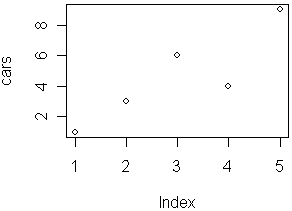
\includegraphics[width=0.7\textwidth]{line_script1.png}
        \caption{Data frame output example}
        \label{fig:dataframe}
    \end{flushleft}
\end{figure}



Let's add a title, a line to connect the points, and some color:

\begin{lstlisting}
# Define the cars vector with 5 values
cars <- c(1, 3, 6, 4, 9)

# Graph cars using blue points overlayed by a line 
plot(cars, type="o", col="blue")

# Create a title with a red, bold/italic font
title(main="Autos", col.main="red", font.main=4)
\end{lstlisting}
\begin{figure}[H]
    \begin{flushleft}
        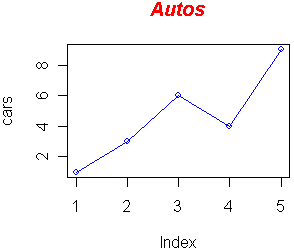
\includegraphics[width=0.7\textwidth]{line_script2.png}
        \caption{Data frame output example}
        \label{fig:dataframe}
    \end{flushleft}
\end{figure}

Now let's add a red line for trucks and specify the y-axis range directly so it will be large enough to fit the truck data:

\begin{lstlisting}
# Define 2 vectors
cars <- c(1, 3, 6, 4, 9)
trucks <- c(2, 5, 4, 5, 12)

# Graph cars using a y axis that ranges from 0 to 12
plot(cars, type="o", col="blue", ylim=c(0,12))

# Graph trucks with red dashed line and square points
lines(trucks, type="o", pch=22, lty=2, col="red")

# Create a title with a red, bold/italic font
title(main="Autos", col.main="red", font.main=4)
\end{lstlisting}

\begin{figure}[H]
    \begin{flushleft}
        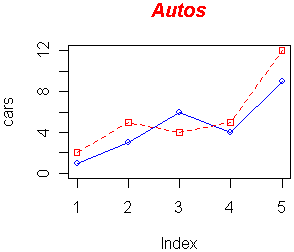
\includegraphics[width=0.7\textwidth]{line_script3.png}
        \caption{Data frame output example}
        \label{fig:dataframe}
    \end{flushleft}
\end{figure}

Next, let's change the axes labels to match our data and add a legend. We'll also compute the y-axis values using the \texttt{max} function so any changes to our data will be automatically reflected in our graph.

\begin{lstlisting}
# Define 2 vectors
cars <- c(1, 3, 6, 4, 9)
trucks <- c(2, 5, 4, 5, 12)

# Calculate range from 0 to max value of cars and trucks
g_range <- range(0, cars, trucks)

# Graph autos using y axis that ranges from 0 to max 
# value in cars or trucks vector.  Turn off axes and 
# annotations (axis labels) so we can specify them ourselves
plot(cars, type="o", col="blue", ylim=g_range, 
   axes=FALSE, ann=FALSE)

# Make x axis using Mon-Fri labels
axis(1, at=1:5, lab=c("Mon","Tue","Wed","Thu","Fri"))

# Make y axis with horizontal labels that display ticks at 
# every 4 marks. 4*0:g_range[2] is equivalent to c(0,4,8,12).
axis(2, las=1, at=4*0:g_range[2])

# Create box around plot
box()

# Graph trucks with red dashed line and square points
lines(trucks, type="o", pch=22, lty=2, col="red")

# Create a title with a red, bold/italic font
title(main="Autos", col.main="red", font.main=4)

# Label the x and y axes with dark green text
title(xlab="Days", col.lab=rgb(0,0.5,0))
title(ylab="Total", col.lab=rgb(0,0.5,0))

# Create a legend at (1, g_range[2]) that is slightly smaller 
# (cex) and uses the same line colors and points used by 
# the actual plots 
legend(1, g_range[2], c("cars","trucks"), cex=0.8, 
   col=c("blue","red"), pch=21:22, lty=1:2)
\end{lstlisting}

\begin{figure}[H]
    \begin{flushleft}
        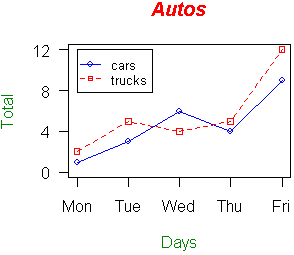
\includegraphics[width=0.7\textwidth]{line_script4.png}
        \caption{Data frame output example}
        \label{fig:dataframe}
    \end{flushleft}
\end{figure}

Now let's read the graph data directly from a tab-delimited file. The file contains an additional set of values for SUVs. We'll save the file in the \texttt{C:/R} directory (you'll use a different path if not using Windows).

\texttt{autos.dat}

\begin{lstlisting}[language=R]
cars trucks suvs
1    2     4
3    5     4
6    4     6
4    5     6
9    12    16
\end{lstlisting}

We'll also use a vector for storing the colors to be used in our graph so if we want to change the colors later on, there's only one place in the file that needs to be modified. Finally, we'll send the figure directly to a PNG file.

\begin{lstlisting}
# Read car and truck values from tab-delimited autos.dat
autos_data <- read.table("C:/R/autos.dat", header=T, sep="\t") 

# Compute the largest y value used in the data (or we could
# just use range again)
max_y <- max(autos_data)

# Define colors to be used for cars, trucks, suvs
plot_colors <- c("blue","red","forestgreen")

# Start PNG device driver to save output to figure.png
png(filename="C:/R/figure.png", height=295, width=300, 
   bg="white")

# Graph autos using y axis that ranges from 0 to max_y.
# Turn off axes and annotations (axis labels) so we can 
# specify them ourselves
plot(autos_data$cars, type="o", col=plot_colors[1], 
   ylim=c(0,max_y), axes=FALSE, ann=FALSE)

# Make x axis using Mon-Fri labels
axis(1, at=1:5, lab=c("Mon", "Tue", "Wed", "Thu", "Fri"))

# Make y axis with horizontal labels that display ticks at 
# every 4 marks. 4*0:max_y is equivalent to c(0,4,8,12).
axis(2, las=1, at=4*0:max_y)

# Create box around plot
box()

# Graph trucks with red dashed line and square points
lines(autos_data$trucks, type="o", pch=22, lty=2, 
   col=plot_colors[2])

# Graph suvs with green dotted line and diamond points
lines(autos_data$suvs, type="o", pch=23, lty=3, 
   col=plot_colors[3])

# Create a title with a red, bold/italic font
title(main="Autos", col.main="red", font.main=4)

# Label the x and y axes with dark green text
title(xlab= "Days", col.lab=rgb(0,0.5,0))
title(ylab= "Total", col.lab=rgb(0,0.5,0))

# Create a legend at (1, max_y) that is slightly smaller 
# (cex) and uses the same line colors and points used by 
# the actual plots
legend(1, max_y, names(autos_data), cex=0.8, col=plot_colors, 
   pch=21:23, lty=1:3)

# Turn off device driver (to flush output to png)
dev.off()
\end{lstlisting}

\begin{figure}[H]
    \begin{flushleft}
        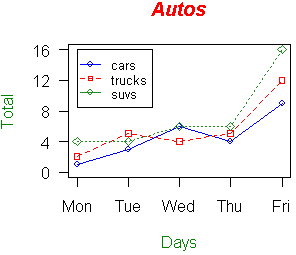
\includegraphics[width=0.7\textwidth]{line_script5.png}
        \caption{Data frame output example}
        \label{fig:dataframe}
    \end{flushleft}
\end{figure}

In this next example, we'll save the file to a PDF and chop off extra white space around the graph; this is useful when wanting to use figures in LaTeX. We'll also increase the line widths, shrink the axis font size, and tilt the x-axis labels by 45 degrees.

\begin{lstlisting}
# Read car and truck values from tab-delimited autos.dat
autos_data <- read.table("C:/R/autos.dat", header=T, sep="\t")

# Define colors to be used for cars, trucks, suvs
plot_colors <- c(rgb(r=0.0,g=0.0,b=0.9), "red", "forestgreen")

# Start PDF device driver to save output to figure.pdf
pdf(file="C:/R/figure.pdf", height=3.5, width=5)

# Trim off excess margin space (bottom, left, top, right)
par(mar=c(4.2, 3.8, 0.2, 0.2))

# Graph autos using a y axis that uses the full range of value
# in autos_data. Label axes with smaller font and use larger 
# line widths.
plot(autos_data$cars, type="l", col=plot_colors[1], 
   ylim=range(autos_data), axes=F, ann=T, xlab="Days",
   ylab="Total", cex.lab=0.8, lwd=2)

# Make x axis tick marks without labels
axis(1, lab=F)

# Plot x axis labels at default tick marks with labels at 
# 45 degree angle
text(axTicks(1), par("usr")[3] - 2, srt=45, adj=1,
          labels=c("Mon", "Tue", "Wed", "Thu", "Fri"),
          xpd=T, cex=0.8)

# Plot y axis with smaller horizontal labels 
axis(2, las=1, cex.axis=0.8)

# Create box around plot
box()

# Graph trucks with thicker red dashed line
lines(autos_data$trucks, type="l", lty=2, lwd=2, 
  col=plot_colors[2])

# Graph suvs with thicker green dotted line
lines(autos_data$suvs, type="l", lty=3, lwd=2, 
  col=plot_colors[3])

# Create a legend in the top-left corner that is slightly  
# smaller and has no border
legend("topleft", names(autos_data), cex=0.8, col=plot_colors, 
   lty=1:3, lwd=2, bty="n")

# Turn off device driver (to flush output to PDF)
dev.off()

# Restore default margins
par(mar=c(5, 4, 4, 2) + 0.1)
\end{lstlisting}

\begin{figure}[H]
    \begin{flushleft}
        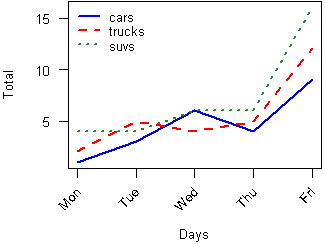
\includegraphics[width=0.7\textwidth]{line_script6.png}
        \caption{Data frame output example}
        \label{fig:dataframe}
    \end{flushleft}
\end{figure}


\section*{Bar Charts}

Let's start with a simple bar chart graphing the \texttt{cars} vector:

\begin{lstlisting}
# Define the cars vector with 5 values
cars <- c(1, 3, 6, 4, 9)

# Graph cars
barplot(cars)
\end{lstlisting}
\begin{figure}[H]
    \begin{flushleft}
        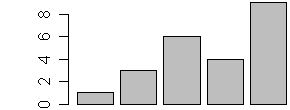
\includegraphics[width=0.7\textwidth]{bar_script1.png}
        \caption{Data frame output example}
        \label{fig:dataframe}
    \end{flushleft}
\end{figure}



\subsection*{Bar Chart with Gray Bars}
Now let's read the auto data from the \texttt{autos.dat} data file, add labels, blue borders around the bars, and density lines:

\begin{lstlisting}
# Read values from tab-delimited autos.dat 
autos_data <- read.table("C:/R/autos.dat", header=T, sep="\t")
   
# Graph cars with specified labels for axes. Use blue 
# borders and diagonal lines in bars.
barplot(autos_data$cars, main="Cars", xlab="Days",  
   ylab="Total", names.arg=c("Mon","Tue","Wed","Thu","Fri"), 
   border="blue", density=c(10,20,30,40,50))
\end{lstlisting}
\begin{figure}[H]
    \begin{flushleft}
        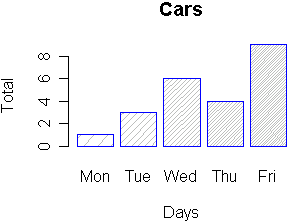
\includegraphics[width=0.7\textwidth]{bar_script2.png}
        \caption{Data frame output example}
        \label{fig:dataframe}
    \end{flushleft}
\end{figure}

\subsection*{Bar Chart with Lined Bars}
Now let's graph the total number of autos per day using some color and show a legend:

\begin{lstlisting}
# Read values from tab-delimited autos.dat 
autos_data <- read.table("C:/R/autos.dat", header=T, sep="\t")
   
# Graph autos with adjacent bars using rainbow colors
barplot(as.matrix(autos_data), main="Autos", ylab= "Total",
   beside=TRUE, col=rainbow(5))

# Place the legend at the top-left corner with no frame  
# using rainbow colors
legend("topleft", c("Mon","Tue","Wed","Thu","Fri"), cex=0.6, 
   bty="n", fill=rainbow(5))
\end{lstlisting}
\begin{figure}[H]
    \begin{flushleft}
        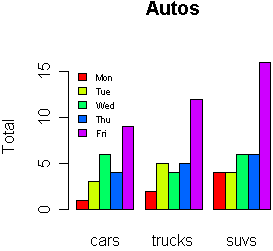
\includegraphics[width=0.7\textwidth]{bar_script3.png}
        \caption{Data frame output example}
        \label{fig:dataframe}
    \end{flushleft}
\end{figure}

\subsection*{Bar Chart with Colorful Bars}
Let's graph the total number of autos per day using a stacked bar chart and place the legend outside of the plot area:

\begin{lstlisting}
# Read values from tab-delimited autos.dat
autos_data <- read.table("C:/R/autos.dat", header=T, sep="\t") 

# Expand right side of clipping rect to make room for the legend
par(xpd=T, mar=par()$mar+c(0,0,0,4))

# Graph autos (transposing the matrix) using heat colors,  
# put 10% of the space between each bar, and make labels  
# smaller with horizontal y-axis labels
barplot(t(autos_data), main="Autos", ylab="Total", 
   col=heat.colors(3), space=0.1, cex.axis=0.8, las=1,
   names.arg=c("Mon","Tue","Wed","Thu","Fri"), cex=0.8) 
   
# Place the legend at (6,30) using heat colors
legend(6, 30, names(autos_data), cex=0.8, fill=heat.colors(3))
   
# Restore default clipping rect
par(mar=c(5, 4, 4, 2) + 0.1)
\end{lstlisting}
\begin{figure}[H]
    \begin{flushleft}
        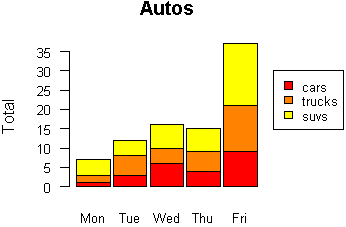
\includegraphics[width=0.7\textwidth]{bar_script4.png}
        \caption{Data frame output example}
        \label{fig:dataframe}
    \end{flushleft}
\end{figure}


\section*{Histograms}

Let's start with a simple histogram graphing the distribution of the \texttt{suvs} vector:

\begin{lstlisting}
# Define the suvs vector with 5 values
suvs <- c(4,4,6,6,16)

# Create a histogram for suvs
hist(suvs)
\end{lstlisting}
\begin{figure}[H]
    \begin{flushleft}
        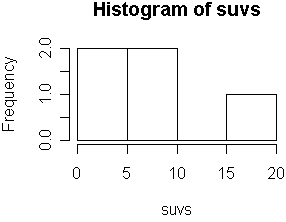
\includegraphics[width=0.7\textwidth]{hist_script1.png}
        \caption{Data frame output example}
        \label{fig:dataframe}
    \end{flushleft}
\end{figure}

\subsection*{Histogram of SUVs with White Bars}
Let's now read the auto data from the \texttt{autos.dat} data file and plot a histogram of the combined car, truck, and SUV data in color.

\begin{lstlisting}
# Read values from tab-delimited autos.dat
autos_data <- read.table("C:/R/autos.dat", header=T, sep="\t")

# Concatenate the three vectors
autos <- c(autos_data$cars, autos_data$trucks, 
   autos_data$suvs)

# Create a histogram for autos in light blue with the y axis
# ranging from 0-10
hist(autos, col="lightblue", ylim=c(0,10))
\end{lstlisting}
\begin{figure}[H]
    \begin{flushleft}
        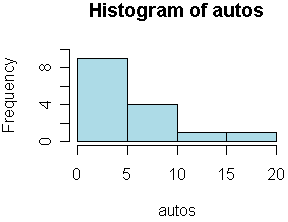
\includegraphics[width=0.7\textwidth]{hist_script2.png}
        \caption{Data frame output example}
        \label{fig:dataframe}
    \end{flushleft}
\end{figure}

\subsection*{Histogram of Autos with Blue Bars}
Now change the breaks so none of the values are grouped together and flip the y-axis labels horizontally.

\begin{lstlisting}
# Read values from tab-delimited autos.dat
autos_data <- read.table("C:/R/autos.dat", header=T, sep="\t")

# Concatenate the three vectors
autos <- c(autos_data$cars, autos_data$trucks, 
   autos_data$suvs)

# Compute the largest y value used in the autos
max_num <- max(autos)

# Create a histogram for autos with fire colors, set breaks
# so each number is in its own group, make x axis range from
# 0-max_num, disable right-closing of cell intervals, set
# heading, and make y-axis labels horizontal
hist(autos, col=heat.colors(max_num), breaks=max_num, 
   xlim=c(0,max_num), right=F, main="Autos Histogram", las=1)
\end{lstlisting}
\begin{figure}[H]
    \begin{flushleft}
        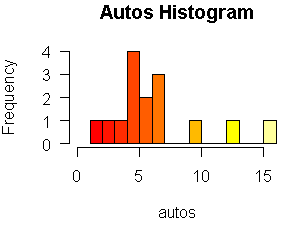
\includegraphics[width=0.7\textwidth]{hist_script3.png}
        \caption{Data frame output example}
        \label{fig:dataframe}
    \end{flushleft}
\end{figure}

\subsection*{Histogram of Autos with Different Groupings}
Now let's create uneven breaks and graph the probability density.

\begin{lstlisting}
# Read values from tab-delimited autos.dat
autos_data <- read.table("C:/R/autos.dat", header=T, sep="\t")

# Concatenate the three vectors
autos <- c(autos_data$cars, autos_data$trucks, 
   autos_data$suvs)

# Compute the largest y value used in the autos
max_num <- max(autos)

# Create uneven breaks
brk <- c(0,3,4,5,6,10,16)

# Create a histogram for autos with fire colors, set uneven
# breaks, make x axis range from 0-max_num, disable right-
# closing of cell intervals, set heading, make y-axis labels 
# horizontal, make axis labels smaller, make areas of each
# column proportional to the count
hist(autos, col=heat.colors(length(brk)), breaks=brk, 
   xlim=c(0,max_num), right=F, main="Probability Density", 
   las=1, cex.axis=0.8, freq=F)
\end{lstlisting}
\begin{figure}[H]
    \begin{flushleft}
        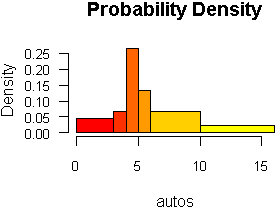
\includegraphics[width=0.7\textwidth]{hist_script4.png}
        \caption{Data frame output example}
        \label{fig:dataframe}
    \end{flushleft}
\end{figure}

\subsection*{Histogram of Autos with Probability Density}
In this example, we'll plot the distribution of 1000 random values that have the log-normal distribution.

\begin{lstlisting}
# Get a random log-normal distribution
r <- rlnorm(1000)

hist(r)
\end{lstlisting}
\begin{figure}[H]
    \begin{flushleft}
        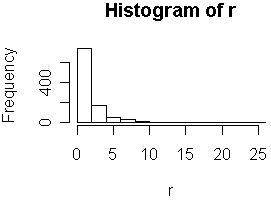
\includegraphics[width=0.7\textwidth]{hist_script5.png}
        \caption{Data frame output example}
        \label{fig:dataframe}
    \end{flushleft}
\end{figure}

\subsection*{Histogram Showing Log-Normal Distribution}
Since log-normal distributions normally look better with log-log axes, let's use the \texttt{plot} function with points to show the distribution.

\begin{lstlisting}
# Get a random log-normal distribution
r <- rlnorm(1000)

# Get the distribution without plotting it using tighter breaks
h <- hist(r, plot=F, breaks=c(seq(0,max(r)+1, .1)))

# Plot the distribution using log scale on both axes, and use
# blue points
plot(h$counts, log="xy", pch=20, col="blue",
	main="Log-normal distribution",
	xlab="Value", ylab="Frequency")
\end{lstlisting}
\begin{figure}[H]
    \begin{flushleft}
        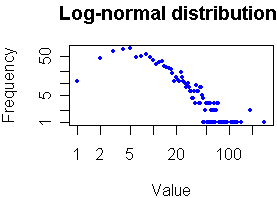
\includegraphics[width=0.7\textwidth]{hist_script6.png}
        \caption{Data frame output example}
        \label{fig:dataframe}
    \end{flushleft}
\end{figure}



\section*{Pie Charts}

Let's start with a simple pie chart graphing the \texttt{cars} vector:

\begin{lstlisting}
# Define cars vector with 5 values
cars <- c(1, 3, 6, 4, 9)

# Create a pie chart for cars
pie(cars)
\end{lstlisting}
\begin{figure}[H]
    \begin{flushleft}
        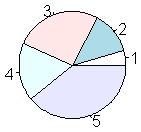
\includegraphics[width=0.7\textwidth]{pie_script1.png}
        \caption{Data frame output example}
        \label{fig:dataframe}
    \end{flushleft}
\end{figure}

\subsection*{Pie Chart of Cars}
Now let's add a heading, change the colors, and define our own labels:

\begin{lstlisting}
# Define cars vector with 5 values
cars <- c(1, 3, 6, 4, 9)

# Create a pie chart with defined heading and
# custom colors and labels
pie(cars, main="Cars", col=rainbow(length(cars)),
   labels=c("Mon","Tue","Wed","Thu","Fri"))
\end{lstlisting}
\begin{figure}[H]
    \begin{flushleft}
        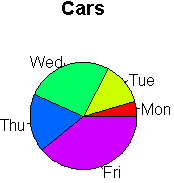
\includegraphics[width=0.7\textwidth]{pie_script2.png}
        \caption{Data frame output example}
        \label{fig:dataframe}
    \end{flushleft}
\end{figure}

\subsection*{Pie Chart with Rainbow Colors}
Now let's change the colors, label using percentages, and create a legend:

\begin{lstlisting}
# Define cars vector with 5 values
cars <- c(1, 3, 6, 4, 9)

# Define some colors ideal for black & white print
colors <- c("white","grey70","grey90","grey50","black")

# Calculate the percentage for each day, rounded to one 
# decimal place
car_labels <- round(cars/sum(cars) * 100, 1)

# Concatenate a '%' char after each value
car_labels <- paste(car_labels, "%", sep="")

# Create a pie chart with defined heading and custom colors
# and labels
pie(cars, main="Cars", col=colors, labels=car_labels,
   cex=0.8)

# Create a legend at the right   
legend(1.5, 0.5, c("Mon","Tue","Wed","Thu","Fri"), cex=0.8, 
   fill=colors)
\end{lstlisting}
\begin{figure}[H]
    \begin{flushleft}
        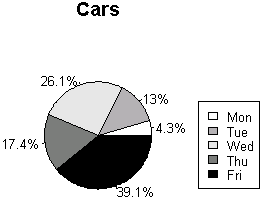
\includegraphics[width=0.7\textwidth]{pie_script3.png}
        \caption{Data frame output example}
        \label{fig:dataframe}
    \end{flushleft}
\end{figure}



\section*{Dotcharts}

Let's start with a simple dotchart graphing the \texttt{autos} data:

\begin{lstlisting}
# Read values from tab-delimited autos.dat
autos_data <- read.table("C:/R/autos.dat", header=T, sep="\t")

# Create a dotchart for autos
dotchart(t(autos_data))
\end{lstlisting}
\begin{figure}[H]
    \begin{flushleft}
        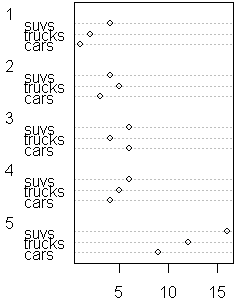
\includegraphics[width=0.7\textwidth]{dot_script1.png}
        \caption{Data frame output example}
        \label{fig:dataframe}
    \end{flushleft}
\end{figure}

\subsection*{Dotchart of autos.dat}
Let's make the dotchart a little more colorful:

\begin{lstlisting}
# Read values from tab-delimited autos.dat
autos_data <- read.table("C:/R/autos.dat", header=T, sep="\t")

# Create a colored dotchart for autos with smaller labels
dotchart(t(autos_data), color=c("red","blue","darkgreen"),
   main="Dotchart for Autos", cex=0.8)
\end{lstlisting}
\begin{figure}[H]
    \begin{flushleft}
        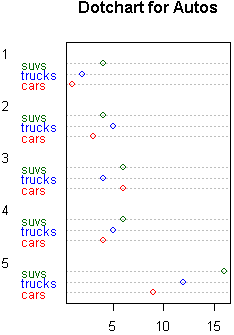
\includegraphics[width=0.7\textwidth]{dot_script2.png}
        \caption{Data frame output example}
        \label{fig:dataframe}
    \end{flushleft}
\end{figure}


\section*{Miscellaneous}

This example shows all 25 symbols that you can use to produce points in your graphs:

\begin{lstlisting}
# Make an empty chart
plot(1, 1, xlim=c(1,5.5), ylim=c(0,7), type="n", ann=FALSE)

# Plot digits 0-4 with increasing size and color
text(1:5, rep(6,5), labels=c(0:4), cex=1:5, col=1:5)

# Plot symbols 0-4 with increasing size and color
points(1:5, rep(5,5), cex=1:5, col=1:5, pch=0:4)
text((1:5)+0.4, rep(5,5), cex=0.6, (0:4))

# Plot symbols 5-9 with labels
points(1:5, rep(4,5), cex=2, pch=(5:9))
text((1:5)+0.4, rep(4,5), cex=0.6, (5:9))

# Plot symbols 10-14 with labels
points(1:5, rep(3,5), cex=2, pch=(10:14))
text((1:5)+0.4, rep(3,5), cex=0.6, (10:14))

# Plot symbols 15-19 with labels
points(1:5, rep(2,5), cex=2, pch=(15:19))
text((1:5)+0.4, rep(2,5), cex=0.6, (15:19))

# Plot symbols 20-25 with labels
points((1:6)*0.8+0.2, rep(1,6), cex=2, pch=(20:25))
text((1:6)*0.8+0.5, rep(1,6), cex=0.6, (20:25))
\end{lstlisting}
\begin{figure}[H]
    \begin{flushleft}
        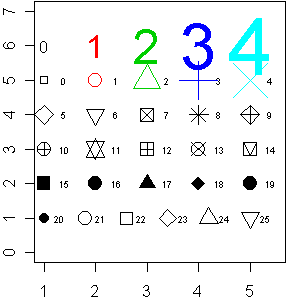
\includegraphics[width=0.7\textwidth]{symbols.png}
        \caption{Data frame output example}
        \label{fig:dataframe}
    \end{flushleft}
\end{figure}

\section*{Exercise Problems: R Graphics}

\subsection*{1. Scatter Plot Customization}
Create a scatter plot with customizations based on the following requirements:
\begin{itemize}
    \item Generate a dataset of 100 random points where \texttt{x} is a sequence of numbers from 1 to 100 and \texttt{y} is normally distributed with a mean of 50 and standard deviation of 10.
    \item Use different colors for points based on whether they are above or below the mean of \texttt{y}.
    \item Add a horizontal line representing the mean of \texttt{y}.
    \item Customize the title, axis labels, and adjust the size of points.
\end{itemize}

\textbf{Bonus:} Use a legend to distinguish points above and below the mean.

\subsection*{2. Grouped Bar Plot of Product Sales}
Using the following data, create a grouped bar plot to compare monthly sales of three products:
\begin{itemize}
    \item \texttt{sales\_data} (Data frame): Product A, Product B, and Product C sales for each month from January to June.
\end{itemize}
Requirements:
\begin{itemize}
    \item Assign unique colors to each product.
    \item Label the x-axis with month names and the y-axis with "Sales".
    \item Add a legend at the top-right corner to indicate each product's color.
\end{itemize}

\textbf{Bonus:} Use a pattern (e.g., diagonal lines, cross-hatching) to differentiate each product in case of black-and-white printing.

\subsection*{3. Pie Chart for Survey Data}
Given the following survey data, create a pie chart representing the distribution of different survey responses:
\begin{itemize}
    \item Survey Responses: \texttt{Satisfied (40\%)}, \texttt{Neutral (35\%)}, and \texttt{Dissatisfied (25\%)}
\end{itemize}
Requirements:
\begin{itemize}
    \item Use distinct colors for each category.
    \item Label each slice with its category name and percentage.
    \item Add a title, and place the legend outside the pie chart.
\end{itemize}

\textbf{Bonus:} Add a custom color palette and adjust label positions to ensure they do not overlap with slices.

\subsection*{4. Histogram of Daily Temperatures}
Using the following temperature data, create a histogram showing the distribution of daily temperatures:
\begin{itemize}
    \item Generate a dataset of 200 random daily temperatures between 60°F and 100°F.
\end{itemize}
Requirements:
\begin{itemize}
    \item Choose an appropriate number of bins to represent the data effectively.
    \item Add color to the histogram bars based on temperature ranges (e.g., \texttt{60-70: blue, 71-80: green, 81-90: orange, 91-100: red}).
    \item Customize the axis labels and title for clarity.
\end{itemize}

\textbf{Bonus:} Add a density curve overlay on the histogram to visualize the distribution more clearly.

\subsection*{5. Box Plot Comparison by Group}
Use the \texttt{iris} dataset to create a box plot comparing \texttt{Sepal.Length} across the different species:
\begin{itemize}
    \item Use different colors for each species.
    \item Customize the y-axis label as "Sepal Length" and the x-axis label as "Species".
    \item Add a title, and make the notches visible for each box.
\end{itemize}

\textbf{Bonus:} Add a summary table beneath the plot showing the mean and median \texttt{Sepal.Length} for each species.






\section*{Control Structures in R: for Loop, while Loop, and if-else Statements}

In R programming, control structures play a vital role in managing the flow of execution, enabling the programmer to repeat tasks, perform actions based on conditions, and more. Here, we delve into three of the most commonly used control structures: the \texttt{for} loop, \texttt{while} loop, and \texttt{if-else} statements.

\section{For Loop in R}

The \texttt{for} loop in R is a control flow statement that allows you to iterate over a sequence (such as a vector, list, or other collections) and execute a block of code for each element in that sequence. This is particularly useful for performing repetitive tasks without manually writing out each iteration.

\subsection{Syntax of the For Loop}

The basic syntax of a \texttt{for} loop in R is as follows:

\begin{lstlisting}[language=R]
for (variable in sequence) {
    % Code to be executed for each element in the sequence
}
\end{lstlisting}

\begin{itemize}
    \item \textbf{variable}: A temporary variable that takes on the value of each element in the sequence during each iteration of the loop.
    \item \textbf{sequence}: This can be a vector, list, or any other collection that you want to iterate over.
\end{itemize}

\subsection{Example 1: Basic For Loop}

Here's a simple example that prints numbers from 1 to 5:

\begin{lstlisting}[language=R]
for (i in 1:5) {
    print(i)
}
\end{lstlisting}

\textbf{Output:}
\begin{lstlisting}[language=R]
[1] 1
[1] 2
[1] 3
[1] 4
[1] 5
\end{lstlisting}

\subsection{Example 2: Calculating the Sum of a Vector}

You can use a \texttt{for} loop to perform calculations, such as summing the elements of a numeric vector:

\begin{lstlisting}[language=R]
numbers <- c(10, 20, 30, 40, 50)
sum_result <- 0

for (num in numbers) {
    sum_result <- sum_result + num
}

print(sum_result)
\end{lstlisting}

\textbf{Output:}
\begin{lstlisting}[language=R]
[1] 150
\end{lstlisting}

\subsection{Example 3: Iterating Over a List}

You can also use a \texttt{for} loop to iterate over elements in a list. Here’s an example that prints the names and ages from a list:

\begin{lstlisting}[language=R]
people <- list(name = c("Alice", "Bob", "Charlie"), age = c(25, 30, 35))

for (i in 1:length(people$name)) {
    cat("Name:", people$name[i], "- Age:", people$age[i], "\n")
}
\end{lstlisting}

\textbf{Output:}
\begin{lstlisting}[language=R]
Name: Alice - Age: 25 
Name: Bob - Age: 30 
Name: Charlie - Age: 35 
\end{lstlisting}

\subsection{Example 4: Creating a Multiplication Table}

You can use a \texttt{for} loop to create a multiplication table for a specific number:

\begin{lstlisting}[language=R]
number <- 7

cat("Multiplication Table for", number, ":\n")
for (i in 1:10) {
    cat(number, "*", i, "=", number * i, "\n")
}
\end{lstlisting}

\textbf{Output:}
\begin{lstlisting}[language=R]
Multiplication Table for 7 :
7 * 1 = 7 
7 * 2 = 14 
7 * 3 = 21 
7 * 4 = 28 
7 * 5 = 35 
7 * 6 = 42 
7 * 7 = 49 
7 * 8 = 56 
7 * 9 = 63 
7 * 10 = 70 
\end{lstlisting}

\subsection{Example 5: Nested For Loops}

You can nest \texttt{for} loops to perform operations on multidimensional data. Here’s an example of creating a 3x3 multiplication table:

\begin{lstlisting}[language=R]
for (i in 1:3) {
    for (j in 1:3) {
        cat(i, "*", j, "=", i * j, "\t")
    }
    cat("\n")  % New line after each row
}
\end{lstlisting}

\textbf{Output:}
\begin{lstlisting}[language=R]
1 * 1 = 1  1 * 2 = 2  1 * 3 = 3  
2 * 1 = 2  2 * 2 = 4  2 * 3 = 6  
3 * 1 = 3  3 * 2 = 6  3 * 3 = 9  
\end{lstlisting}

\subsection{Example 6: Using a For Loop with Conditional Statements}

You can incorporate \texttt{if} statements inside a \texttt{for} loop to filter values. For example, to print only even numbers from a vector:

\begin{lstlisting}[language=R]
numbers <- 1:10

for (num in numbers) {
    if (num %% 2 == 0) {
        cat(num, "is even\n")
    }
}
\end{lstlisting}

\textbf{Output:}
\begin{lstlisting}[language=R]
2 is even
4 is even
6 is even
8 is even
10 is even
\end{lstlisting}

\subsection{Summary}

The \texttt{for} loop in R is a powerful tool for automating repetitive tasks, whether you are performing calculations, processing lists, or generating formatted outputs. By understanding how to use \texttt{for} loops effectively, you can enhance your data manipulation and analysis capabilities in R.

\section{While Loop in R}

The \texttt{while} loop in R is a control flow structure that allows you to repeat a block of code as long as a specified condition evaluates to \texttt{TRUE}. It is useful when the number of iterations is not predetermined and depends on dynamic conditions evaluated at runtime.

\subsection{Syntax of \texttt{while} Loop}

The basic syntax for a \texttt{while} loop in R is as follows:

\begin{lstlisting}[language=R]
while (condition) {
  # Code to be executed repeatedly
}
\end{lstlisting}

\begin{itemize}
    \item \textbf{condition}: A logical expression that is evaluated before each iteration. If the condition is \texttt{TRUE}, the loop continues; if it is \texttt{FALSE}, the loop stops.
    \item The code block within the braces \{\} will be executed repeatedly as long as the condition remains \texttt{TRUE}.
\end{itemize}

\subsection{Characteristics of \texttt{while} Loop}

\begin{itemize}
    \item The condition is checked \textbf{before} executing the loop body, which means if the condition is \texttt{FALSE} from the beginning, the loop body will not execute at all.
    \item It is crucial to ensure that the condition will eventually evaluate to \texttt{FALSE} to avoid creating an infinite loop.
\end{itemize}

\subsection{Examples of \texttt{while} Loop}

\subsubsection{1. Basic Countdown}

This example demonstrates a simple countdown from 10 to 1.

\begin{lstlisting}[language=R]
countdown <- 10
while (countdown > 0) {
  print(countdown)
  countdown <- countdown - 1
}
print("Liftoff!")
\end{lstlisting}

\textbf{Explanation}:
\begin{itemize}
    \item The loop starts with \texttt{countdown} set to 10.
    \item It prints the value of \texttt{countdown} and then decrements it by 1 until it reaches 0.
    \item Once \texttt{countdown} is 0, it exits the loop and prints "Liftoff!"
\end{itemize}

\subsubsection{2. User Input Until Condition Met}

In this example, we will prompt the user to enter numbers until they enter a negative number.

\begin{lstlisting}[language=R]
sum <- 0
number <- 0

while (number >= 0) {
  number <- as.numeric(readline(prompt = "Enter a number (negative to stop): "))
  sum <- sum + number
}
cat("Total sum:", sum, "\n")
\end{lstlisting}

\textbf{Explanation}:
\begin{itemize}
    \item The loop continues as long as the user enters a non-negative number.
    \item The numbers entered by the user are summed up, and when a negative number is entered, the loop terminates, and the total sum is printed.
\end{itemize}

\subsubsection{3. Collatz Conjecture}

This example implements the Collatz Conjecture using a \texttt{while} loop.

\begin{lstlisting}[language=R]
collatz_steps <- function(n) {
  steps <- 0
  while (n != 1) {
    if (n %% 2 == 0) {
      n <- n / 2  # If n is even
    } else {
      n <- 3 * n + 1  # If n is odd
    }
    steps <- steps + 1
  }
  return(steps)
}

number <- 7
cat("Number of steps for", number, "to reach 1:", collatz_steps(number), "\n")
\end{lstlisting}

\textbf{Explanation}:
\begin{itemize}
    \item The function \texttt{collatz\_steps} takes a positive integer \texttt{n} and applies the Collatz rules until \texttt{n} becomes 1.
    \item The number of steps taken is counted and returned.
\end{itemize}

\subsubsection{4. Infinite Loop with Exit Condition}

Here’s an example of creating a loop that runs indefinitely until a certain condition is met.

\begin{lstlisting}[language=R]
repeat {
  response <- readline(prompt = "Type 'exit' to stop: ")
  if (response == "exit") {
    cat("Exiting the loop.\n")
    break  # Exit the loop
  }
  cat("You typed:", response, "\n")
}
\end{lstlisting}

\textbf{Explanation}:
\begin{itemize}
    \item This loop will keep running until the user types "exit".
    \item The \texttt{break} statement is used to exit the loop when the condition is met.
\end{itemize}

\subsection{Important Notes}
\begin{itemize}
    \item Be cautious when using \texttt{while} loops to avoid infinite loops. Ensure that there is a clear exit condition and that the condition will eventually be met.
    \item Use \texttt{break} to exit the loop prematurely based on a specific condition if necessary.
    \item You can combine \texttt{while} loops with other control flow statements (like \texttt{if} statements) to create complex logic as required by your application.
\end{itemize}

\subsection{Conclusion}

The \texttt{while} loop is a powerful and flexible tool in R that allows for repetitive execution of code based on dynamic conditions. Understanding how to use it effectively is essential for programming in R, especially for tasks that require iterative processes based on user input or calculated conditions.

\section{If-Else Statements in R}

The \textbf{if-else statement} in R is a fundamental control structure that allows you to execute different blocks of code based on specific conditions. This is particularly useful for decision-making within your code, enabling you to respond differently to varying inputs or situations.

\subsection{Basic Structure}

The basic syntax of an if-else statement in R is as follows:

\begin{lstlisting}[language=R]
if (condition) {
  # Code to execute if the condition is TRUE
} else {
  # Code to execute if the condition is FALSE
}
\end{lstlisting}

\subsection{Explanation of Components}

\begin{itemize}
    \item \textbf{condition}: This is a logical expression that evaluates to either \texttt{TRUE} or \texttt{FALSE}. If the condition is \texttt{TRUE}, the code within the first block is executed. If it's \texttt{FALSE}, the code within the \texttt{else} block is executed.
    
    \item \textbf{Code Blocks}: The code inside the \{\} braces is the block of code that gets executed based on the evaluation of the condition. You can have multiple lines of code in each block.
\end{itemize}

\subsection{Extended If-Else Statement}

You can also extend the if-else structure using \texttt{else if} to handle multiple conditions:

\begin{lstlisting}[language=R]
if (condition1) {
  # Code to execute if condition1 is TRUE
} else if (condition2) {
  # Code to execute if condition2 is TRUE
} else {
  # Code to execute if all conditions are FALSE
}
\end{lstlisting}

\subsection{Examples}

\subsubsection{Example 1: Basic If-Else}

\begin{lstlisting}[language=R]
x <- 10

if (x > 5) {
  print("x is greater than 5")
} else {
  print("x is less than or equal to 5")
}
\end{lstlisting}

\textbf{Output:}
\begin{lstlisting}[language=R]
[1] "x is greater than 5"
\end{lstlisting}

In this example, since \texttt{x} is 10, the condition \texttt{x > 5} evaluates to \texttt{TRUE}, and the corresponding message is printed.

\subsubsection{Example 2: If-Else with Multiple Conditions}

\begin{lstlisting}[language=R]
x <- 15

if (x < 10) {
  print("x is less than 10")
} else if (x >= 10 && x < 20) {
  print("x is between 10 and 20")
} else {
  print("x is 20 or more")
}
\end{lstlisting}

\textbf{Output:}
\begin{lstlisting}[language=R]
[1] "x is between 10 and 20"
\end{lstlisting}

In this example, \texttt{x} is 15, which satisfies the second condition (\texttt{x >= 10 \&\& x < 20}), so the corresponding message is printed.

\subsubsection{Example 3: Checking for Even or Odd}

\begin{lstlisting}[language=R]
num <- 7

if (num %% 2 == 0) {
  print("The number is even.")
} else {
  print("The number is odd.")
}
\end{lstlisting}

\textbf{Output:}
\begin{lstlisting}[language=R]
[1] "The number is odd."
\end{lstlisting}

Here, the modulus operator (\texttt{\%\%}) checks if \texttt{num} is even or odd. Since 7 is not divisible by 2, the message indicates it is odd.

\subsubsection{Example 4: Grading System}

\begin{lstlisting}[language=R]
score <- 85

if (score >= 90) {
  grade <- "A"
} else if (score >= 80) {
  grade <- "B"
} else if (score >= 70) {
  grade <- "C"
} else if (score >= 60) {
  grade <- "D"
} else {
  grade <- "F"
}

print(paste("Your grade is:", grade))
\end{lstlisting}

\textbf{Output:}
\begin{lstlisting}[language=R]
[1] "Your grade is: B"
\end{lstlisting}

In this grading example, the score is evaluated against several thresholds to determine the corresponding letter grade.




\subsubsection{Example 5: Using Logical Operators}

\begin{lstlisting}[language=R]
age <- 25
has_license <- TRUE

if (age >= 18 && has_license) {
  print("You can drive.")
} else {
  print("You cannot drive.")
}
\end{lstlisting}

\textbf{Output:}
\begin{lstlisting}[language=R]
[1] "You can drive."
\end{lstlisting}

In this example, both the age and license status are checked. Since the conditions are met, the message indicates that the user can drive.

\subsection{Summary}

If-else statements are a powerful tool in R programming, allowing for conditional execution of code based on logical conditions. They can be used in various scenarios, from simple checks to complex decision-making processes. By using \texttt{if}, \texttt{else if}, and \texttt{else}, you can create more sophisticated logic flows in your R scripts.



\section*{Exercise Problems}

\subsection*{1. For Loop Exercises}

\begin{enumerate}
    \item \textbf{Sum of Squares}
    \begin{itemize}
        \item Write a \texttt{for} loop that calculates the sum of the squares of the integers from 1 to 20 and prints the result.
    \end{itemize}

    \item \textbf{Fibonacci Sequence}
    \begin{itemize}
        \item Generate the first 10 Fibonacci numbers using a \texttt{for} loop and print them in a single line.
    \end{itemize}

    \item \textbf{Factorial Calculation}
    \begin{itemize}
        \item Create a \texttt{for} loop that calculates the factorial of a given number \( n \) (e.g., \( n = 5 \)) and print the result.
    \end{itemize}

    \item \textbf{Multiplication Table}
    \begin{itemize}
        \item Using a \texttt{for} loop, create a multiplication table for the number 7 (from 1 to 10) and print it in a formatted way.
    \end{itemize}

    \item \textbf{Character Count}
    \begin{itemize}
        \item Write a \texttt{for} loop that counts the number of vowels in a given string (e.g., ``Hello, World!'') and prints the count.
    \end{itemize}
\end{enumerate}

\subsection*{2. While Loop Exercises}

\begin{enumerate}
    \item \textbf{Countdown}
    \begin{itemize}
        \item Write a \texttt{while} loop that counts down from 10 to 1 and prints each number. Print ``Liftoff!'' after reaching 0.
    \end{itemize}

    \item \textbf{Sum of Numbers}
    \begin{itemize}
        \item Create a \texttt{while} loop that continually asks the user to input numbers until they enter a negative number. Calculate and print the sum of the entered numbers (excluding the negative number).
    \end{itemize}

    \item \textbf{Collatz Conjecture}
    \begin{itemize}
        \item Implement the Collatz Conjecture using a \texttt{while} loop: Starting from a positive integer \( n \), keep applying the following rules until \( n \) becomes 1:
        \begin{itemize}
            \item If \( n \) is even, divide it by 2.
            \item If \( n \) is odd, multiply it by 3 and add 1.
        \end{itemize}
        Print the number of steps taken to reach 1.
    \end{itemize}

    \item \textbf{Guess the Number}
    \begin{itemize}
        \item Write a simple number guessing game using a \texttt{while} loop. Randomly generate a number between 1 and 100, and prompt the user to guess the number. Provide feedback on whether their guess is too high or too low, and continue until they guess correctly.
    \end{itemize}

    \item \textbf{Infinite Loop Control}
    \begin{itemize}
        \item Write a \texttt{while} loop that runs indefinitely and prints ``Running...'' until the user types ``stop''. Use \texttt{readline()} to capture user input to control the loop.
    \end{itemize}
\end{enumerate}

\subsection*{3. If-Else Statement Exercises}

\begin{enumerate}
    \item \textbf{Even or Odd}
    \begin{itemize}
        \item Write a program that checks if a number input by the user is even or odd, and prints the result.
    \end{itemize}

    \item \textbf{Grade Calculator}
    \begin{itemize}
        \item Create a program that takes a numerical score (0 to 100) from the user and prints the corresponding letter grade based on the following scale:
        \begin{itemize}
            \item A: 90-100
            \item B: 80-89
            \item C: 70-79
            \item D: 60-69
            \item F: below 60
        \end{itemize}
    \end{itemize}

    \item \textbf{Age Checker}
    \begin{itemize}
        \item Write an \texttt{if-else} statement that checks a person's age and prints whether they are a child (0-12), teenager (13-19), adult (20-64), or senior (65+).
    \end{itemize}

    \item \textbf{Discount Eligibility}
    \begin{itemize}
        \item Create a program that checks if a customer is eligible for a discount based on their membership status (member or non-member) and the total purchase amount (e.g., discounts for members over \$50).
    \end{itemize}

    \item \textbf{Password Strength Checker}
    \begin{itemize}
        \item Write an \texttt{if-else} statement to check the strength of a password based on the following criteria:
        \begin{itemize}
            \item Length: at least 8 characters
            \item Contains at least one uppercase letter
            \item Contains at least one lowercase letter
            \item Contains at least one digit
        \end{itemize}
        Print whether the password is strong, moderate, or weak based on these criteria.
    \end{itemize}
\end{enumerate}

\subsection*{Additional Challenge Problems}

\begin{enumerate}
    \item \textbf{Combining Control Structures}
    \begin{itemize}
        \item Write a program that takes a list of numbers (e.g., from 1 to 50) and uses a \texttt{for} loop and an \texttt{if} statement to print only the prime numbers from that list.
    \end{itemize}

    \item \textbf{Pattern Printing}
    \begin{itemize}
        \item Create a nested \texttt{for} loop that prints the following pattern:
        \begin{lstlisting}[language=R]
        *
        **
        ***
        ****
        *****
        \end{lstlisting}
    \end{itemize}

    \item \textbf{Bank Account Simulation}
    \begin{itemize}
        \item Implement a simple bank account simulation where a user can deposit or withdraw money. Use a \texttt{while} loop to continue prompting the user until they choose to exit. Use \texttt{if-else} statements to handle invalid transactions (e.g., overdrafts).
    \end{itemize}
\end{enumerate}

This code uses a simple enumerated list without specifying labels, which should resolve the issue you encountered. You can now copy and paste this into your LaTeX document. Let me know if you need any further adjustments!









\section{Working with Packages}
Packages enhance R's capabilities, providing additional functions.
\begin{itemize}
    \item How to find and use R packages.
    \item Overview of essential packages for statistics (e.g., \texttt{MASS}, \texttt{caret}, \texttt{tidyverse}).
    \item How to check package documentation and help files.
\end{itemize}

\section{R Markdown}
R Markdown is a powerful tool for creating dynamic reports.
\begin{itemize}
    \item Creating dynamic reports that combine code and output.
    \item Exporting reports to different formats (HTML, PDF, Word).
\end{itemize}





















\title{Calculating Weighted Mean for Grouped Data}

\section*{Calculating Weighted Mean for Grouped Data}
Suppose you have a dataset representing a set of observations, and you want to analyze the distribution of values within specific class intervals. The data points are divided into intervals, and you want to calculate the weighted mean using the midpoints of these intervals.

\begin{enumerate}
  \item \textbf{Given Data:}
    \begin{itemize}
      \item A set of data points: $\{5, 15, 25, 35, 45, 55, 65\}$.
      \item Class intervals defined as $0, 10, 20, 30, 40, 50, 60, 70$ with a step size of 10.
    \end{itemize}
    
  \item \textbf{Objective:}
    \begin{itemize}
      \item Utilize the provided R code to create class intervals, calculate midpoints, and determine the weighted mean for the grouped data.
    \end{itemize}
    
  \item \textbf{Procedure:}
    \begin{itemize}
      \item Use the \texttt{cut} function in R to categorize the data into intervals based on the specified class intervals.
      \item Calculate the midpoints of these intervals.
      \item Compute the weighted mean using the formula $\frac{\sum (f \cdot x)}{\sum f}$, where $f$ is the frequency and $x$ is the midpoint of the interval.
    \end{itemize}
    
  \item \textbf{Results:}
    \begin{itemize}
      \item Display the resulting data frame, showing the original data points along with their corresponding class intervals.
      \item Print the calculated weighted mean using the midpoints.
    \end{itemize}
    
  \item \textbf{Conclusion:}
    \begin{itemize}
      \item Interpret the results and draw conclusions about the distribution of the data within the defined intervals.
    \end{itemize}
\end{enumerate}

\section*{R Code}
\begin{lstlisting}[language=R, caption={R Code for Calculating Weighted Mean}, label={lst:weighted_mean}]
# Create some example data
data <- c(5, 15, 25, 35, 45, 55, 65)

# Define the class intervals
class_intervals <- seq(0, 70, by = 10)

# Use cut to create intervals
interval_labels <- cut(data, breaks = class_intervals,

 include.lowest = TRUE, right = FALSE)

# Calculate midpoints
midpoints <- (class_intervals[-1] + 

class_intervals[-length(class_intervals)]) / 2

# Calculate the weighted mean
weighted_mean <- sum(midpoints * table(interval_labels)) / length(data)

# Display the result
data_frame <- data.frame(Data = data, Class_Interval = interval_labels)
print(data_frame)

# Print the mean using midpoints
cat("Weighted Mean using Midpoints:", weighted_mean, "\n")
\end{lstlisting}

\subsection{Exercise}

Write an R program to find the median and mode of continuously grouped data.

\newpage


\section{Correlation}

Correlation analysis is a statistical technique used to measure the strength and direction of a linear relationship between two variables. In this lab, we will explore correlation using the R programming language. The dataset used for this analysis contains two variables, denoted as \(X\) and \(Y\). The primary objectives include loading and exploring the dataset, calculating and interpreting the correlation coefficient, visualizing the relationship through a scatter plot, and conducting a significance test on the correlation coefficient.

\section{Objectives}

\begin{enumerate}
    \item \textbf{Load and Explore the Dataset:} The dataset used for this analysis contains two variables, denoted as \(X\) and \(Y\). The first step is to load the data into R and explore its characteristics.
    
    \begin{lstlisting}[language=R]
    # Load the dataset
    data <- read.csv("correlation_data.csv")
    
    # Display the first few rows of the dataset
    head(data)
    
    # Summary statistics
    summary(data)
    \end{lstlisting}
    
    \item \textbf{Exploratory Data Analysis (EDA):} Upon loading the dataset, we examine its structure and summary statistics to gain insights into the distribution and nature of the variables.
    
    \begin{itemize}
        \item \textbf{Descriptive Statistics:} The summary statistics provide information about the central tendency, dispersion, and shape of the distributions of variables \(X\) and \(Y\).
        
        \item \textbf{Correlation Calculation:} Next, we calculate the correlation coefficient (\(r\)) to quantify the strength and direction of the linear relationship between \(X\) and \(Y\).
        
        \begin{lstlisting}[language=R]
        # Calculate the correlation coefficient
        correlation_coefficient <- cor(data$X, data$Y)
        \end{lstlisting}
    \end{itemize}
    
    \item \textbf{Scatter Plot Visualization:} To enhance our understanding, a scatter plot is created to visualize the relationship between \(X\) and \(Y\).
    


    

        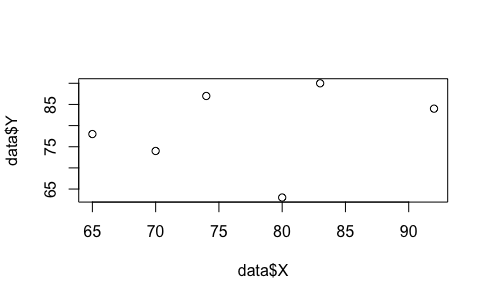
\includegraphics[width=0.8\textwidth]{scatter_plot.png}

    
    
\end{enumerate}

\section{Results}

\subsection{Correlation Coefficient}

The calculated correlation coefficient (\(r\)) between \(X\) and \(Y\) is \texttt{correlation\_coefficient}.

\subsection{Scatter Plot}

The scatter plot visually represents the relationship between \(X\) and \(Y\). The plot indicates the direction and strength of the correlation (see Figure \ref{fig:scatter_plot}).

\section{Discussion}

The interpretation of the correlation coefficient and the scatter plot should be discussed. Consider the implications of the results in the context of the dataset. Questions to address include:

\begin{itemize}
    \item Is the correlation positive or negative?
    \item What is the strength of the correlation?
    \item How do outliers or influential points affect the interpretation?
\end{itemize}


\newpage


\section{Regression}

Linear regression is a widely used statistical technique that aims to model the relationship between a dependent variable and one or more independent variables. It assumes a linear relationship and is commonly employed for predicting outcomes based on given inputs. This lab explores the principles of linear regression using the R programming language, a powerful tool for statistical analysis.

\section{Objectives}

\begin{enumerate}
    \item \textbf{Understand Linear Regression:} Grasp the fundamental concepts behind linear regression and its applications.
    \item \textbf{Perform Regression Analysis in R:} Learn how to implement linear regression using R programming.
    \item \textbf{Interpret Results:} Develop skills to interpret and draw meaningful conclusions from regression analysis outcomes.
\end{enumerate}

\section{Materials and Methods}

\subsection{Data Collection}

A dataset was utilized containing information on the hours of study and exam scores of a group of students. The dataset was loaded into R, and its structure and initial rows were examined.

\begin{lstlisting}[language=R]
# Load the dataset
data <- read.csv("study_data.csv")

# Display the structure of the dataset
str(data)

# Display the first few rows of the dataset
head(data)
\end{lstlisting}

\subsection{Linear Regression Analysis}

Linear regression analysis was performed using the \texttt{lm()} function in R, taking "ExamScore" as the dependent variable and "HoursOfStudy" as the independent variable.

\begin{lstlisting}[language=R]
# Perform linear regression
model <- lm(ExamScore ~ HoursOfStudy, data = data)

# Display the summary of the regression model
summary(model)
\end{lstlisting}

\section{Results}

\subsection{Descriptive Statistics}

Before interpreting regression results, descriptive statistics for the variables were examined.

\begin{lstlisting}[language=R]
# Display summary statistics for HoursOfStudy
summary(data$HoursOfStudy)

# Display summary statistics for ExamScore
summary(data$ExamScore)
\end{lstlisting}

\subsection{Regression Coefficients}

The regression coefficients were inspected to understand the relationship between the hours of study and exam scores.

\begin{lstlisting}[language=R]
# Display regression coefficients
coefficients(model)
\end{lstlisting}

\subsection{Model Summary}

The summary of the regression model was analyzed, including key statistics such as R-squared, F-statistic, and p-values.

\begin{lstlisting}[language=R]
# Display model summary
summary(model)
\end{lstlisting}

\section{Discussion}

\subsection{Interpretation of Coefficients}

The coefficient for "HoursOfStudy" represents the estimated change in the dependent variable ("ExamScore") for a one-unit change in the independent variable. In our case, this coefficient indicates the average change in exam score for each additional hour of study.

\subsection{Model Fit}

The R-squared value indicates the proportion of the variance in the dependent variable that is predictable from the independent variable. A higher R-squared suggests a better fit of the model to the data.

\section{Conclusion}

This lab introduced the principles of linear regression and demonstrated its implementation in R. By exploring the relationship between hours of study and exam scores, valuable insights were gained. The interpretation of coefficients, assessment of model fit, and hypothesis testing provided a comprehensive understanding of the dataset.


\newpage



\title{Lab Report: Large Sample Test on a Single Mean in R}
\section{Introduction}

The large sample test on a single mean is a statistical technique used to assess whether the mean of a single sample significantly differs from a known or hypothesized population mean. This lab aims to demonstrate the application of such a test using the R programming language.

\section{Objectives}

\begin{enumerate}
    \item \textbf{Understand Large Sample Testing:} Comprehend the principles of large sample tests on a single mean.
    \item \textbf{Conduct Hypothesis Testing in R:} Learn how to perform large sample tests using R.
    \item \textbf{Interpret Results:} Develop skills to interpret and draw meaningful conclusions from hypothesis testing outcomes.
\end{enumerate}

\section{Materials and Methods}

\subsection{Data Collection}

A dataset was collected or loaded into R, containing a sample of interest. The characteristics of this dataset were examined to understand its distribution and key statistics.

\begin{lstlisting}[language=R]
# Load the dataset
data <- read.csv("sample_data.csv")

# Display the structure of the dataset
str(data)

# Display summary statistics
summary(data)
\end{lstlisting}

\subsection{Large Sample Test}

A large sample test on a single mean was performed using the appropriate test function in R. The null hypothesis typically assumes that the sample mean is equal to a specified population mean.

\begin{lstlisting}[language=R]
# Perform large sample test on a single mean
result <- t.test(data$Variable, mu = 50)

# Display the test result
print(result)
\end{lstlisting}

\section{Results}

\subsection{Descriptive Statistics}

Before conducting the large sample test, descriptive statistics for the variable of interest were examined.

\begin{lstlisting}[language=R]
# Display summary statistics for the variable
summary(data$Variable)
\end{lstlisting}

\subsection{Large Sample Test Results}

The results of the large sample test were analyzed, including test statistics, degrees of freedom, and p-values.

\begin{lstlisting}[language=R]
# Display the test result
print(result)
\end{lstlisting}

\section{Discussion}

\subsection{Interpretation of Results}

Interpret the results of the large sample test, considering the calculated test statistic and p-value. Discuss the implications of these results in the context of the research question.

\subsection{Practical Significance}

Consider whether the observed difference, if statistically significant, is also practically significant. Discuss the real-world implications of the findings.

\subsection{Assumptions and Limitations}

Highlight any assumptions made during the analysis and acknowledge any limitations that might affect the validity of the results.

\section{Conclusion}

Summarize the key findings of the large sample test on a single mean and draw conclusions based on the analysis. Discuss the relevance of the results to the original research question.














% Appendix
%\appendix
%\chapter{Appendix A: LaTeX Resources}
%Here are some useful resources to help you further explore LaTeX:
%
%\begin{itemize}
%    \item \href{https://www.latex-project.org/}{LaTeX Project Official Website}
%    \item \href{https://www.overleaf.com/learn}{Overleaf LaTeX Documentation}
%\end{itemize}
%
%\index{Resources} % Adding to the index
%
%\chapter{Appendix B: Common LaTeX Errors}
%When working with LaTeX, you may encounter common errors like missing braces or improper package usage. Refer to the following resources for troubleshooting:
%
%\begin{itemize}
%    \item StackExchange: \url{https://tex.stackexchange.com/}
%    \item LaTeX Wikibook: \url{https://en.wikibooks.org/wiki/LaTeX}
%\end{itemize}
%
%\index{Errors} % Adding to the index

% Bibliography
\newpage
\printbibliography
\addcontentsline{toc}{chapter}{Bibliography}

% Example of a sample .bib entry in the references.bib file:
% @book{lamport1994latex,
%   title={LaTeX: A document preparation system},
%   author={Lamport, Leslie},
%   year={1994},
%   publisher={Addison-Wesley}
% }

% Index
\newpage
\addcontentsline{toc}{chapter}{Index} % Ensure the index appears in the TOC
\printindex

\end{document}